\documentclass[12pt]{article}

\usepackage[T1]{fontenc}
\usepackage[dvips,letterpaper,margin=0.75in,bottom=0.75in]{geometry}
\usepackage{cite}
%\usepackage{slashed}
\usepackage{cancel}
\usepackage{graphicx}
\usepackage{amsmath}
\usepackage{braket}
\usepackage{latexsym,amssymb,amsmath}
\usepackage{pdfpages}
\usepackage{xcolor}
\usepackage{capt-of}

\usepackage[american,fulldiode]{circuitikz}
\tikzset{component/.style={draw,thick,circle,fill=white,minimum size =0.75cm,inner sep=0pt}}

\begin{document}
\ctikzset{bipoles/thickness=1}
\ctikzset{bipoles/length=.6cm}

\title{Proposal for Revising the \\ Undergraduate Physics Curriculum \\ Version 1.14}
\author{Undergraduate Curriculum Committee}

\maketitle

\section{TODO}
\begin{itemize}
 \item Update example syllabi to match faculty meeting presentations.
 \item Fix the prereq table.
 \item Follow up with Rena
 \item Find Tony comments?
\end{itemize}


\section{Changes Since the Previous Version}
This proposal has been updated since the previous version based on
feedback from the assigned faculty reviews and any other comments
which have been received.
\begin{itemize}  
 \item The contents of the example course syllabi of
   Section~\ref{sec:syllabi} have been revised based on the
   presentations at the (first) annual faculty curriculum review.
\end{itemize}

\newpage

\tableofcontents

\newpage

\section{Objectives of the Proposal}

An example schedule of student course work without the revisions
proposed here is shown in Table~\ref{tbl:current-honors} for students
taking honors physics.  An example schedule for students that transfer
to UC Davis for their junior year is shown in
Table~\ref{tbl:current-transfers}.  There are many different
trajectories through our program, but most are some variation on these
two.  For consistent comparisons, all the example schedules in this
proposal assume the students take 122A and one capstone course in the
winter, and two capstone courses in the spring.  Many other lab
courses and offerings are possible.

\captionof{table}{\label{tbl:current-honors} An example schedule
  satisfying the {\em current requirements} for an undergraduate
  physics major that takes the 9H series and 122A. Physics course
  numbers are shown with the number of units in parenthesis.  Math
  courses start with M.  Courses in italics are electives or have at
  least two different offerings per year. Course CAP is a capstone
  elective, and course X is any advanced elective.}
\begin{center}
\begin{tabular}{|l|l|l|l|}
\hline
Year      & Fall    & Winter & Spring \\
\hline
Freshman  & 9HA(5)     & 9HB(5)     & 9HC(5) \\
          & {\it M21B(4)}  & {\it M21C(4)}  & {\it M21D(4)} \\
\hline
Sophomore & 9HD(5)     & 9HE(5)     & 40(4)     \\
          & {\it M22A(3)}     & {\it M22B(3)} & {\it 80(4)} \\
\hline
Junior    & 104A(4) & 105B(4) & 110B(4)\\
          & 105A(4) & 110A(4) & 115A(4)\\
          & 102(1)  &    &     \\
\hline
Senior    & 110C(4) & {\it 122A(4)} & {\it X(3-4)}\\
          & 112(4)  & {\it CAP(4)}   & {\it X(3-4)}\\
          & 115B(4) & {\it CAP(4)}   & {\it CAP(4)}\\

\hline 
\end{tabular}
\end{center}

\captionof{table}{\label{tbl:current-transfers} An example schedule
  satisfying the {\em current requirements} for an undergraduate
  physics major that transfers to UC Davis in their junior year and
  takes 122A.  Physics course numbers are shown with the number of
  units in parenthesis.  Courses in italics are electives or have at
  least two different offerings per year.  Course CAP is a capstone
  elective, and course X is any advanced elective.  Note that PHY 102
  is generally considered to be much more work than a typical one-unit
  course.}
\begin{center}
\begin{tabular}{|l|l|l|l|}
\hline
Year      & Fall    & Winter & Spring \\
\hline
Junior    & 9D(4)   & 105B(4) & 40(4)   \\
          & 104A(4) & 110A(4) & 110B(4) \\
          & 105A(4) & {\it 80(4)}   & 115A(4) \\
          & 102(1)  &         & \\
\hline
Senior    & 110C(4) & {\it 122A(4)} & {\it X(3-4)}\\
          & 112(4)  & {\it CAP(4)}   & {\it X(3-4)}\\
          & 115B(4) & {\it CAP(4)}   & {\it CAP(4)}\\
\hline 
\end{tabular}
\end{center}

There are some deficiencies in the current course of study:
\begin{itemize}

\item Physics majors who complete 9HD or 9D in the fall of their
  sophomore year have little to do for the rest of the year.  The
  honors sequence has 9HE, but that course does not contain any
  content which is a prequisite for upper division class work.  The
  recent addition of 40 and 80 is helpful in that it provides
  something for students to do during this time, but the problem still
  remains that they do not make progress on the upper division core
  course work, and 80 is not taken by all students.  The result of
  this stalling is that the junior and senior year are a race to
  complete the degree requirements, leaving very little flexibility or
  time for advanced electives.

\item Students that transfer to UC Davis for their junior year face a
  wall of course work that they have to handle in the first quarter:
  math methods, mechanics, and modern physics.  Many also take 102,
  which is nominally a one-unit course, but generally nearly as much
  work as a four-unit course.  For many students, these are also the
  first courses they encounter that require solving challenging
  homework problems.  We have two trains of students running through
  our program and the fall of their junior year is the train wreck
  where they collide.

\item The current curriculum does not include sufficient computing
  practice for our students.  It is useful to consider what a physics
  degree would look like if we taught calculus the same way we teach
  computing.  Students would arrive their freshman year and take an
  introductory calculus course.  Then, they would take their physics
  courses, which would never mention calculus.  At some point in their
  junior or senior year, they would take a one quarter course called
  ``Calculus in Physics'' which would attempt to show all the ways we
  use calculus in physics.  Our students are experts at calculus
  because they learn how to use the tool, and then apply it, again and
  again, throughout their course work.  To remain relevant in the
  modern world (or even the world from 20 years ago) our majors need
  more practice in the use of computing as an essential tool for
  solving physics problems.

\item Four-year students typically graduate with around 180 units.
  Within the College of Letters and Science, we are allowed to require
  a maximum of 110 units in our majors.  The current BS physics major
  requires a minimum of 108 units to complete.  Fitting the canon of
  undergraduate physics into such a tight space is extremely
  challenging.  Students complain that we waste time teaching some
  topics again and again (e.g. Special Relativity from scratch) while
  completely dropping other topics (e.g. Classical Hamiltonians).  The
  problem is particularly acute for applied physics majors, where core
  material must be dropped to make space for course work outside of
  physics.

\item The prerequisite structure of the upper division courses creates
  many tiers.  As an extreme example, 122 requires 112, which requires
  115A, which requires 104A and 105A, both of which require the 9
  series.  This, combined with the rapid pace, leaves very little
  flexibility for students once they start their junior year.  For
  example, missing any of the four-unit courses in the junior year of
  Table~\ref{tbl:current-honors} requires an exception to
  prerequisites or an extra year to graduate.
\end{itemize}
This proposal aims to make significant improvements on each of these issues.

\newpage

\section{Proposed BS Requirements}

The proposed required courses for a BS in physics are presented in
Tables~\ref{tbl:prep} and \ref{tbl:depth}.  Example schedules are
presented in
Tables~\ref{tbl:proposed-honors}-\ref{tbl:proposed-transfers}.

A primary feature of this proposal is that incoming transfer students
now overlap in some courses with sophomores that took the honors
physics sequence.  This eliminates the stalling of our four-year
students while relieving some of the intense academic pressure on
incoming transfer students.  Our experience has been that the best of
our transfer students perform as well as the best of our four-year
students, once they have sufficient time to adjust, and this proposal
gives them that time.  Accelerating students that took the honors
sequence also provides tremendous additional flexibility to their
schedule.  The example schedule in Table~\ref{tbl:proposed-honors}
assumes the student takes each class nearly as soon as possible,
leaving ample time in their senior year for additional electives.

Transfer students that wish to complete their degree in two years are
still highly constrained, but instead of facing three upper division
courses immediately upon arrival they now start with one upper
division course.  Take the time to compare fall quarter of the junior
year in Tables~\ref{tbl:current-transfers} and
\ref{tbl:proposed-transfers}, this is a major feature of this
proposal.  This gentle introduction does not come at the cost of
dramatically increased unit loads later on: transfer students can
still complete the degree without exceeding 13 units of physics
course work in any quarter.

The college imposes a limit of 110 units of required course work,
including prerequisites, for any major.  Within a particular major,
options that exceed this limit are permitted, as long as a path that
stays below the limit is available.  The current BS physics major
requires a minimum of 108 units.  This proposal takes advantage of the
remaining two units and brings the minimum to 110 units.  This
slightly increases total unit pressure on students, which particularly
affects those transfer students who have only two-years to absorb
them.  However, the proposal replaces the one-unit course PHY 102 with
the more accurately credited four-unit PHY 45 course.  Also, the major
stress point for transfer students is in their first quarter, which
this proposal substantially improves.  The proposal also adds
significantly more schedule flexibility, which should also help
alleviate pressure.

\newpage

\vskip 2cm
\captionof{table}{\label{tbl:prep}Preparatory Subject Matter}
\noindent
\vskip 0.25cm
Units:  53-54. *: recommended, $\parallel$ concurrently\\
\begin{tabular}{|llllll|}
\hline
Course & & Units & Offered & Prereqs & Name \\
\hline
MAT & 21A & 4 & FWS & & Differential Calculus\\ 
    & 21B & 4 & FWS & 21A & Integral Calculus \\ 
    & 21C & 4 & FWS & 21B & Partial Derivatives and Series\\ 
    & 21D & 4 & FWS & 21C & Vector Analysis\\ 
    & 22A & 3 & FWS & 21C & Linear Algebra\\ 
    & 22B & 3 & FWS & 22A & Differential Equations\\ 
\hline
\hline

PHY & 9A & 5 & FS & 21B & Classical Physics {\it (Class. Mech.)}\\ 
    & 9B & 5 & FW & 9A,21C & Classical Physics {\it (Waves, Thermo., Optics.)}\\ 
    & 9C & 5 & WS & 9B,21D & Classical Physics {\it (Elec. and Magn.)}\\ 
    & 9D & 4 & FS & 9C,22A & Modern Physics {\it (Rel. and Quant. Mech.)}\\ 
\hline
&or&&\\
\hline
PHY & 9HA & 5 & F & $\parallel$21B/$\parallel$21M & Honors Physics {\it (Class. Mech.)}\\ 
    & 9HB & 5 & W & 21B/21M & Honors Physics {\it (Rel. and Stat. Mech.)}\\ 
    & 9HC & 5 & S & 21C & Honors Physics {\it (Waves and Quant. Mech.)}\\ 
    & 9HD & 5 & F & 21D & Honors Physics {\it (Elec. and Magn.)}\\ 
\hline
\hline
PHY & 40  & 4 & F & & Introduction to Physics Computation \\ 
    & 45  & 4 & W & 40,9C/9HD,$\parallel$22B & Computational Physics\\ 
    & 80  & 4 & WS & 40$\dagger$,9C/9HD     & Experimental Techniques \\
PHY & 185* & 1 & S & & Careers in Physics \\ 
    & 190* & 1 & F & & Careers in Physics \\ 
\hline
\end{tabular}
$\dagger$:  Instructor permission may be obtained to take PHY 80 without the PHY 40 prerequisite.


\newpage
\captionof{table}{\label{tbl:depth}Depth Subject Matter}
\noindent
\vskip 0.25cm
Units:  42-46. *: recommended, $\parallel$: concurrently.\\
\begin{tabular}{|llllll|}
\hline
Course & & Units & Offered & Prereqs & Name \\
\hline
PHY & 104A & 4 & FS & 9C/9HD,MAT 22B   & Mathematical Physics \\ 
    & 105A & 4 & W & 9C/9HD,$\parallel$MAT 22B & Classical Mechanics I\\
    & 105B & 4 & S & 105A,40$\dagger$          & Classical Mechanics II\\ 
    & 110A & 4 & W & 104A             & Electricity and Magnetism I\\
    & 110B & 4 & S & 110A,9HD/$\parallel$9D    & Electricity and Magnetism II\\
    & 112  & 4 & F & 104A,9D/9HD      & Thermodynamics and Stat. Mech.\\    
    & 115A & 4 & F & 104A,105A,9D/9HD & Quantum Mechanics I \\
    & 115B & 4 & W & 115A             & Quantum Mechanics II \\
    & 115C* & 4 & S & 115B,45/ECS 36B& Applications of Quantum Mechanics\\ 
\hline
\hline
PHY & 116A & 4 &  F & 80              & Phys. Instr. with A\&D Electronics.  \\
    & 116B & 4 &  W & 80,45/ECS 36B   & Phys. Instr. for Data Acquisition. \\ 
\hline
    & or & & & & \\
\hline
PHY & 122A/B & 4 & WS & 80,104A,105A,110B & Advanced Physics Laboratory \\  
    &  & & & \& $\parallel$112 $\parallel$115A&  \\  

\hline
\hline
 & Any two of & & & & (all three recommended): \\
\hline 
PHY & 110L & 1 & S & 45/ECS 36B, $\parallel$110B & Comp. Lab in Electricity and Magn. \\
    & 112L & 1 & F & 45/ECS 36B, $\parallel$112  & Comp. Lab in Statistical Mechanics \\ 
    & 115L & 1 & W & 45/ECS 36B, $\parallel$115B & Comp. Lab in Quantum Mechanics \\ 
\hline
\end{tabular}\\ \vskip 0.25cm
\noindent
$\dagger$:  Instructor permission may be obtained to take PHY 105B without the PHY 40 prerequisite.
\noindent
{\bf Electives:} Additional electives to bring the total number of 3-4 unit upper division courses to 14, including at least three from capstone courses.  
(3-4 courses, totaling 12-16 units with current offerings)
\\
\noindent
{\bf Total Units:} 110-112

\newpage
\captionof{table}{ An example schedule satisfying the
  {\em proposed requirements} for an undergraduate physics major that
  takes the 9H series and 122A. Physics course numbers are shown with
  the number of units in parenthesis.  Math courses start with M.
  Courses in italics are electives or have at least two different
  offerings per year. Course CAP is a capstone elective, and course X
  is any advanced elective.  Rate is 3-9 physics units per quarter in
  junior and senior year.}
\label{tbl:proposed-honors}
\begin{center}
\begin{tabular}{|l|l|l|l|}
\hline
Year      & Fall    & Winter & Spring \\
\hline
Freshman  & 9HA(5)       & 9HB(5)        & 9HC(5) \\
          & {\it M21B(4)} & {\it M21C(4)}  & {\it M21D(4)}\\
\hline
Sophomore & 9HD(5)       & 105A(4)      & 105B(4) \\
          & {\it M22A(3)} & {\it M22B(3)} & {\it 104A(4)} \\
          & 40(4)        & 45(4)       & {\it 80(4)}  \\
\hline
Junior    & 115A(4) & 115B+L(5)  & {\it 115C(4)}\\
          & 112+L(5)  & 110A(4)  & 110B+L(5)\\
\hline
Senior    & {\it X(3-4)} & {\it 122A(4)} & {\it CAP(4)} \\
          &              & {\it CAP(4)} & {\it CAP(4)} \\
\hline  
\end{tabular}
\end{center}


\vskip 2cm
\captionof{table}{ An example schedule satisfying the
  {\em proposed requirements} for an undergraduate physics major that
  takes the 9 series and 122A. Physics course numbers are shown with
  the number of units in parenthesis.  Math courses start with M.
  Courses in italics are electives or have at least two different
  offerings per year. Course CAP is a capstone elective, and course X
  is any advanced elective.  Rate is 7-13 physics units per quarter in
  junior and senior year.}
\label{tbl:proposed-nonhonors}
\begin{center}
\begin{tabular}{|l|l|l|l|}
\hline
Year      & Fall    & Winter & Spring \\
\hline
Freshman  & {\it M21A(4)}  & {\it M21B(4)}  & {\it M21C(4)}\\
          &               &               & {\it 9A(5)} \\
\hline
Sophomore & {\it M21D(4)}  & {\it M22A(3)}  & {\it M22B(3)}\\ 
          & {\it 9B(5)}    & {\it 9C(5)}    & {\it 9D(4)} \\
          & 40(4)          &                & {\it 80(4)} \\
\hline
Junior   & {\it 104A(4)}   & 105A(4)       & 105B(4) \\
         & {\it X(3-4)}      & 110A(4)       & 110B+L(5) \\         
         &                 & 45(4)         & \\

\hline
Senior   & 115A(4)    & 115B+L(5)     & {\it 115C(4)} \\
         & 112+L(5)   & {\it 122A(4)} & {\it CAP(4)} \\
         &            & {\it CAP(4)}   & {\it CAP(4)}  \\
\hline 
\end{tabular}
\end{center}

\newpage
\captionof{table}{An example schedule satisfying the
  {\em proposed requirements} for an undergraduate physics major that
  transfers to UC Davis in their junior year, without Physics 9D or 40
  equivalents, and takes 122A. Physics course numbers are shown with
  the number of units in parenthesis.  Courses in italics are
  electives or have at least two different offerings per year. Course
  CAP is a capstone elective, and course X is any advanced elective.
  Rate is 12-13 units per quarter.  Note that only one upper division
  course is required in the first quarter of junior year, compared to
  three upper division courses in the current program.  }
\label{tbl:proposed-transfers}
\begin{center}
\begin{tabular}{|l|l|l|l|}
\hline
Year      & Fall    & Winter & Spring \\
\hline
Junior   & 9D(4)         & 105A(4)   & 105B(4) \\
         & 40(4)         & 110A(4)   & 110B+L(5) \\         
         & {\it 104A(4)} & 45(4)     & {\it 80(4)} \\
\hline
Senior   & 115A(4)    & 115B+L(5)      & {\it 115C(4)} \\
         & 112+L(5)   & {\it 122A(4)} & {\it CAP(4)} \\
         & {\it X(3-4)} & {\it CAP(4)}   & {\it CAP(4)}  \\
\hline 
\end{tabular}
\end{center}


Several new courses have been added, some are no longer offered, and
others require changes to their content:
\begin{itemize}
\begin{samepage}
\item 9A-D and 9HA-D are largely unchanged, however, some fine
  adjustments may be needed to ensure that the 9 series plus 104A are
  sufficient preparation for 112.  Also, there are some minor
  adjustments to the math prerequisites.
\end{samepage}

\item 9HE is no longer offered.  This course is effectively an
  elective, with content that varies from instructor to instructor.
  By removing it, we allow the students in the honors sequence to
  start toward the core material sooner, leaving more time for
  advanced electives. With the more relaxed schedule in their senior
  year, it seems highly plausible that physics majors will take more
  advanced electives.

\item 104A: This course will now be offered in both fall and spring,
  as discussed further in the discussion of prerequisites.  Most
  students taking honors physics will take the course in the spring,
  while most transfer students will take the course in the fall.  Two
  offerings will remove a major bottleneck, result in smaller class sizes,
  and will allow the course to be pitched slightly differently in
  these two quarters, to better reflect student preparation.

\item 105: The timing of the 105AB sequence is adjusted to start in
  winter.  The content of 105AB should be at a level appropriate for a
  sophomore completing 9HD in the previous quarter.  There is no prerequisite for
  104A, but typically students will take 104A either concurrently with
  105B or before 105A.

\item 110: The present curriculum devotes three quarters of required
  upper division course work to Electricity and Magnetism (110ABC).
  This proposal eliminates 110C and increases the pace of 110AB.
  Students must reliably enter 110 having adequate preparation in
  vector calculus, curvilinear coordinates, Lorentz transformation,
  relativistic mechanics, and introductory electricity and magnetism.
  This material must be covered adequately in the 9 series and 104A.


\item 112: The 115A prerequisite for 112 has been removed, and the
  treatment must rely on quantum from the PHY 9 series instead.  PHY 9
  and 9H must both reliably cover discrete energy levels from the
  particle in a box and simple harmonic oscillator.  Fermi and Bose
  statistics will need to be introduced independently in 112.
  
\item The 115AB sequence is extended to include an elective third
  quarter: 115C.  The prerequisites are 104A and 105A.  The elective
  third quarter, 115C, adds 45 as a prerequisite, and the course
  includes extensive computational problems.  The extra time should
  also allow coverage of new elective topics (for example Quantum
  Information Theory).

\item 45, 110L, 112L, and 115L: PHY 45 is a new required four-unit
  course in computational physics.  Students are also required to take
  at least two of three new one-unit computing lab courses 110L, 112L,
  and 115L.  These courses are discussed in more detail in
  Section~\ref{sec:comp}.

\item 102 and 104B: these computational courses will no longer be
  offered and will no longer be required for any major.

\item The 116ABC sequence adds PHY 80 as a prerequisite and is reduced
  to a two quarter sequence 116AB.  In the current program, there is
  significant duplication of PHY 80 content in PHY 116A and PHY 116C,
  so no content is lost in this reorganization.  The lab courses are
  discussed in detail in Section~\ref{sec:labs}.
\end{itemize}
Example syllabi for the new required courses and existing courses
affected by this proposal are presented in Section~\ref{sec:syllabi}.

This proposal is approximately neutral with respect to the cost of
instruction if we assume that the cost of electives is held constant
(we of course have no obligation to do so.)  The second offering of
104A, the new required course 45, and the new required one unit
computing labs add a total of three new instructors.  But dropping
courses 9HE, 102, 104B, 110C and 116C frees 4.3 instructors, for a net
decrease of 1.3 instructors.  If the need for more sections of 80
requires an additional instructor (currently typically two, although
three were initially planned for 2020-2021) there would be a decrease
of 0.3 instructors.  Additional fall offerings for 122A/B could be
added as well, if needed to meet demand.

\section{Theoretical Physics}
\label{sec:theory}

At the core of any undergraduate physics degree are the following
topics in theoretical physics:
\begin{itemize}
\item Classical Mechanics (105AB): the fundamental principles of physical laws
  (e.g. least action and symmetries) are taught in a familiar and
  intuitive context. 
\item Electromagnetism (110AB): a remarkable special case of classical
  phenomenon that anticipates non-Newtonian physics (e.g. special
  relativity, gauge theories).  No other force in nature can be understood so
  completely in such a straight forward fashion.  
\item Quantum Mechanics (115AB): the rules governing the microscopic world are
  different from those governing our familiar macroscopic world.  The
  rules are not intuitive but they can be codified and used to make
  quantitative predictions which can be experimentally verified.
\item Statistical Mechanics (112): provides the crucial statistical explanation for how
  microscopic laws ultimately produce the macroscopic world which we inhabit.
\end{itemize}
This proposal includes a procedure for maintaining example syllabi for
the core courses to ensure these topics are being consistently and
effectively covered.  While this proposal need not resolve all of the
issues, a digest of the current discussion is provided here:
\begin{itemize}
 \item It is generally agreed that 105A needs to cover Hamiltonian mechanics, but this has not been managed reliably.
 \item We need to find a consistent location to cover the calculus of variations.
 \item There is support for covering waveguides in 110AB.
   Waveguides are a possible topic for 110L (not taken by every
   student) They could also be added to 80 with an experimental focus
   (which will be taken by every student).
 \item The treatment of radiation in 110AB is limited.
 \item PHY 104A plays a central role in providing students with the
   analytic techniques needed for upper division course work.  This
   course has been far too topical for the central role it plays in
   our program.   
 \item While this proposal doesn't include any changes to PHY 115AB, but we should develop and discuss example syllabi for this course along with the other core courses.
\end{itemize}
Example syllabi are presented in Section~\ref{sec:syllabi}.  

\section{Computational Physics}
\label{sec:computing}

\begin{figure}
\begin{center}
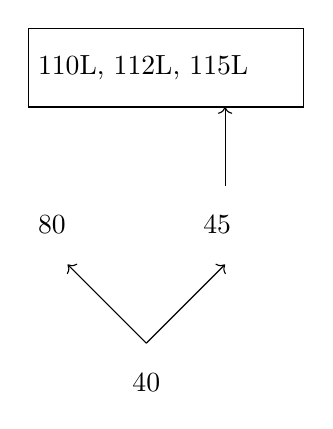
\begin{tikzpicture}

% 1st tier:
\node[right] at (1.2,0.5) {40};
%\draw (0,0) coordinate(X) -- ++(0,1) -- ++(1.8,0) |- (X);

\draw[->] (1.5,1) --(0.5,2);
\draw[->] (1.5,1) --(2.5,2);


% 2nd tier:
\node[right] at (0,2.5) {80};
%\draw (0,2) coordinate(X) -- ++(0,1.0) -- ++(1.2,0) |- (X);

\node[right] at (2.1,2.5) {45};

\draw[->] (2.5,3) --(2.5,4);

% 3rd tier:
\draw (0,4.0) coordinate(X) -- ++(0,1) -- ++(3.5,0) |- (X);
\node[right] at (0,4.5) {110L, 112L, 115L};

\end{tikzpicture}

\caption{\label{fig:comps} Prerequisite structure of computational courses.}

\end{center}
\end{figure}

One of the major objectives of this proposal is to better integrate
computational physics throughout the curriculum.  To do so, students
must have a consistent set of tools that can be relied upon in later
courses.  The course descriptions in the course catalog will not
reference specific tools, to allow this to evolve over time, but in a
consistent manner.  In this proposal, the supported computational
tools are:
\begin{itemize}
\item Scientific computing tools for Python: NumPy, SciPy, MatPlotLib,
  and Jupyter Notebooks via Anaconda
\item C/C++
\item Computer Algebra:  Mathematica or SymPy
\end{itemize}
The entire Scientific Python ecosystem is easily accessible to
students for any major OS for free through Anaconda.  No graphical
features of C/C++ will be explored.  If necessary, C++ programs will
pass data by text file to SciPy for plotting.  SymPy is not as mature
as Mathematica, but comes with the significant advantages of being
freely available within Anaconda and interoperable with SciPy.

In 2018, we added a new required course, PHY 40, which introduces
programming with both C++ and python.  This format leaves no time for
symbolic computation and little time for exploring additional features
of Scientific Python beyond the basic Python language.  This proposal
modifies the computational content of existing courses and adds
several new required courses:
\begin{itemize}
\item 40: This four-unit course, which has no prerequisites and
  assumes no prior knowledge of programing, provides an introduction
  to programming using examples from computational physics.  It
  includes a short introduction to symbolic manipulations using a
  computer algebra system.  The specific tools covered (which will not
  be included in the course description) are Scientific Python and
  either SymPy or Mathematica.

\item 45: This new four-unit course, Computational Physics, will have
  the PHY 9 series through E\&M as a prerequisite (9C/9HD) as well as
  PHY 40.  PHY 45 will replace the requirement for 102 or 104B.  The
  focus will be on solving physics problems at the conceptual level of
  the 9 series using computational physics.  It will introduce the C++
  programming language and continue using Scientific Python.
  
\item 80: is a new four-unit lab course introduced in 2018 which
  includes extensive use of scientific python for data analysis and
  presentation, including curve fitting and plotting scientific data.
  In this proposal, 80 is required for all majors.  It adds 40 as a
  prerequisite, but with an exception intended for AB majors as described
  in Section ~\ref{sec:ab}.

\item 110L, 112L, and 115L: These three new one-unit computational lab
  courses are designed to be taken concurrently with 110B, 112, and
  115B. They are computational problem solving labs related to E\&M,
  statistical mechanics, and quantum mechanics.  The emphasis will be
  on solving problems from upper division physics using computing at
  the level of PHY 45.  One unit courses should involve three hours of
  academic work per week as described below.  One instructor could
  teach all three of these courses in a single year, which would count
  toward instructor workload as a single three unit course.  Each course
  is offered in a different quarter, so students get three units of
  computational problem-solving spread across an entire year.  Due to
  unit limits, we only require two of these courses, but all three are
  recommended.

\item 105B: this course now has PHY 40 as a prerequisite and can
  therefore include computational problems in mechanics using
  Scientific Python or computer algebra.

\item 115C: This new elective course has PHY 45 as a prerequisite and
  is intended to include extensive computational problem solving as an
  integral part of the course.
  
\end{itemize}
Physics BS majors will be required to take 18 units (23 recommended)
of course work that involves extensive computing exercises.
Furthermore, once student computing abilities are on more solid
ground, capstone and advanced elective courses could further evolve to
include additional computing exercises and add 45 (or at least 40) as
a prerequisite.  All applied majors include 45 or an equivalent, so,
for example, even 140A could include a computational component.

{\bf One-unit workload: }It is important that 110L, 112L, and 115L are
taught as one-unit courses.  A one-unit course should involve three
hours of total academic work per week, which in this case includes the
one hour of scheduled lecture time.  For example, an appropriate
workload would be five computing assignments due every two weeks
during the ten week quarter.  Each assignment would be introduced with
a one-hour lecture, with a second one-hour lecture devoted to helping
students complete the assignment.  The assignments should take about
five hours to complete, including one hour of help.

\section{Lab Course Work}
\label{sec:labs}

In traditional lab courses, students conduct scientific experiments,
gain crucial hands on experience, and see theoretical concepts from a
new perspective.  The unit cap on required coursework places extreme
time pressure on these essential lab experiences: BS physics majors
are only required to take four units of upper division traditional lab
work, although many opt to take more.

Physics 80 was introduced in 2018, and is currently a prerequisite for
Physics 122A/B.  It is anticipated that this will relieve some of the
intense time pressure in these courses.  The 122 labs cycle students
through experimental stations, and enrollment in each quarter is
limited by the number of available stations.  This proposal makes some
adjustments to the prerequisites of 122A/B which would allow for fall
offerings.  This will help meet the expected increase in demand for
122A/B due to increased enrollment.  As can be seen in
Table~\ref{tbl:proposed-honors}, many seniors have room to take 122A/B
in the fall of their senior year.  We also plan to add additional
stations to 122A/B, which is independent from this proposal.

In this proposal, Physics 80 is also added as a prerequisite for the
116 (Instrumentation) sequence as well.  Physics 80 covers some of the
content in current versions of 116A (passive analog electronics) and
116C (computation with scientific python and statistical analysis).
Therefore, the three quarter 116 sequence (A,B, and C) becomes a two
quarter sequence, with 116A covering analog and digital electronics,
and 116B covering data acquisition with microprocessors and FPGAs.
For additional flexibility, 116B no longer has 116A as a prerequisite,
as sufficient analog electronics is covered in 80.

Physics 80 and 116 share the same dedicated lab space.  The primary
time for taking 80 will be in spring quarter, but it will also be
offered in fall, and possibly winter, while 116A and 116B will be
offered in fall and winter respectively.  The department plans to
expand the lab space available for 80 and 116 to meet the needs of
increase enrollment.

\section{Prerequisites}

\begin{figure}
\begin{center}
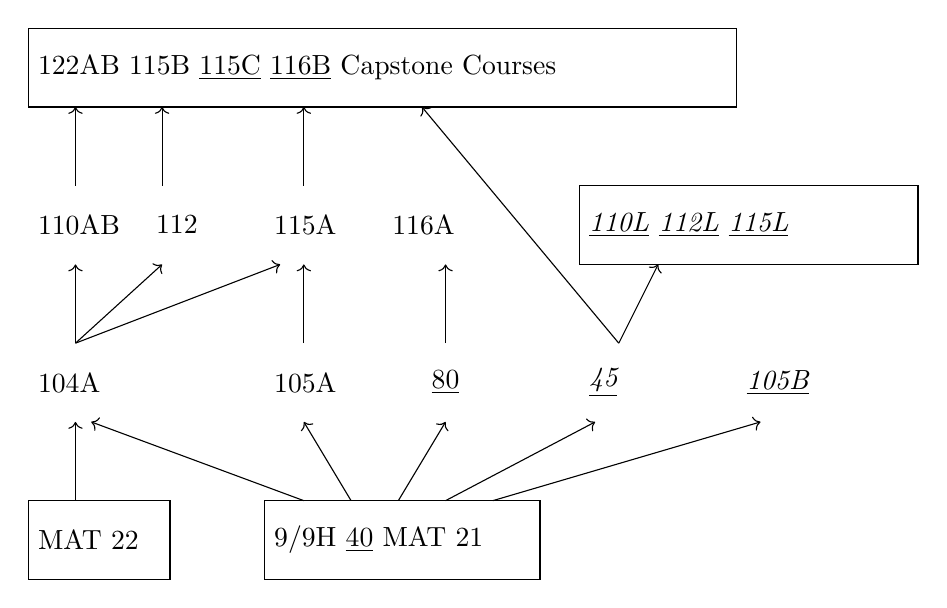
\begin{tikzpicture}

% 1st tier:
\node[right] at (0,0.5) {MAT 22};
\draw (0,0) coordinate(X) -- ++(0,1) -- ++(1.8,0) |- (X);

\node[right] at (3,0.5) {9/9H \underline{40} MAT 21};
\draw (3,0) coordinate(X) -- ++(0,1) -- ++(3.5,0) |- (X);



\draw[->] (0.6,1) --(0.6,2);
\draw[->] (3.5,1) --(0.8,2);
\draw[->] (4.1,1) --(3.5,2);
\draw[->] (4.7,1) --(5.3,2);
\draw[->] (5.3,1) --(7.2,2);
\draw[->] (5.9,1) --(9.3,2);
%\draw[->] (7.4,1) --(7.4,2);
%\draw[->] (7.2,1) --(5.5,2);


% 2nd tier:
\node[right] at (0,2.5) {104A};
%\draw (0,2) coordinate(X) -- ++(0,1.0) -- ++(1.2,0) |- (X);

\node[right] at (3,2.5) {105A};

\node[right] at (5,2.5) {\underline{80}};

\node[right] at (7,2.5) {\it \underline{45}};

\node[right] at (9,2.5) {\it \underline{105B}};

\draw[->] (0.6,3) --(0.6,4);
\draw[->] (0.6,3) --(1.7,4);
\draw[->] (0.6,3) --(3.2,4);

\draw[->] (3.5,3) --(3.5,4);

\draw[->] (5.3,3) --(5.3,4);

\draw[->] (7.5,3) --(5,6);
\draw[->] (7.5,3) --(8.0,4);


% 3rd tier:
\node[right] at (0,4.5) {110AB};

\node[right] at (1.5,4.5) {112};

\node[right] at (3,4.5) {115A};

\node[right] at (4.5,4.5) {116A};

\node[right] at (7,4.5) {\it \underline{110L} \underline{112L} \underline{115L}};
\draw (7,4) coordinate(X) -- ++(0,1) -- ++(4.3,0) |- (X);

\draw[->] (0.6,5) --(0.6,6);
\draw[->] (1.7,5) --(1.7,6);
\draw[->] (3.5,5) --(3.5,6);


% top tier:
\node[right] at (0,6.5) {122AB 115B {\underline{115C}} {\underline{116B}} Capstone Courses};
\draw (0,6) coordinate(X) -- ++(0,1) -- ++(9.0,0) |- (X);


\end{tikzpicture}

\caption{\label{fig:prereqs} {\color{red} NEEDS WORK???} Consider adding years...
  The prerequisite structure of physics and related math courses.
  Courses within a box may have an internal prerequisite structure not
  shown.  For clarity, in some cases only the most advanced
  prerequisites are shown.  Prerequisites within a sequence (e.g. 112L
  has concurrent prerequisite with 112) are not shown.  All required
  courses are shown.  Underlined courses have a significantly
  computational component.  Italicized courses are required for a BS
  in Physics but can be safely omitted from the Astrophysics major, as
  they do not serve as prerequisites for other required courses in
  that major.}
\end{center}
\end{figure}

An overview of the prerequisite structure is shown in
Fig.~\ref{fig:prereqs}.  The graph reveals 104A as a major bottleneck
in our program, as it requires the most advanced material from the
first tier (MAT 22) but is required for most upper division classes,
such as 110A and 115A.  The committee spent a great deal of time
considering different ways to relieve or accommodate this bottleneck
but in the end decided two offerings is the only effective way to
achieve the goals of this proposal.  This stems from the fact that
incoming transfer students must start on 104A immediately upon arrival
in fall to complete the remaining upper division courses in two years,
but sophomores finishing 9HD in the fall are not generally ready to
take 104A until the spring.

It appears from the graph that 45 is a potential bottleneck as well,
but it is less severe.  It does not require MAT 22A so can be taken
sooner than 104A, and it is only needed for top tier courses such as
115C and the computational lab courses, which can be postponed until
senior year.

The most notable changes to the prerequisite structure are:
\begin{itemize}
\item 80 adds 40 as a prerequisite, with an exception for AB majors as described in Section~\ref{sec:ab}.

\item 112 does not require 115A anymore, 104A and 9A-D must suffice
  instead.  
\item 110A does not require 105A anymore. 
\item 105B requires 40, so computational examples can be used in this course.
\item 122A/B adds a 115A prerequisite, which was implicit when 115A was a prerequisite for 112.  Both 112 and 115A are allowed to be concurrent, which will not be possible unless we add a fall offering of 122.
\end{itemize}

The new prerequisite structure is considerably more flexible.  In the
junior year of Tables~\ref{tbl:proposed-nonhonors} and
\ref{tbl:proposed-transfers} missing or failing 104A or 105A
jeopardizes a timely graduation, but instructor permission from one
course (110A or 115A) will allow the student to proceed on schedule.
The situation in Table~\ref{tbl:proposed-honors} is even more
forgiving.

\newpage

\section{Proposed BS with Specialization in Astrophysics}
The Astrophysics specialization requires updates to the prerequisites
for PHY 151-158, mainly to accommodate the new schedule which offers
PHY 105A in the fall and to add PHY 40 as a new required course.  The
Astrophysics specialty courses now include 158, for a total of five,
from which four are chosen.  Limits on the number of units precludes
including PHY 45, and the related lab courses, to the program.
However, the PHY 151-158 courses have already begun to include
extensive computational physics directly related to astrophysics.

The proposed required courses for the Astrophysics specialization are presented in
Tables~\ref{tbl:prep-astro-applied} and \ref{tbl:depth-astro}.  To avoid
version conflicts, some information in Tables \ref{tbl:prep} and
\ref{tbl:depth} is not duplicated in these tables.  Example schedules are presented
in Table~\ref{tbl:proposed-astro}.

\captionof{table}{\label{tbl:prep-astro-applied}Preparatory Subject Matter:  Astrophysics and Applied Physics}
\noindent
\vskip 0.25cm
\begin{center}
Units:  49-50. *: recommended, $\parallel$: concurrently.\\
\begin{tabular}{|lll|}
\hline
Course & & Units \\
\hline
MAT & 21A & 4 \\  
    & 21B & 4 \\ 
    & 21C & 4 \\ 
    & 21D & 4 \\ 
    & 22A & 3 \\ 
    & 22B & 3 \\ 
\hline
\hline
PHY & 9A & 5 \\  
    & 9B & 5 \\  
    & 9C & 5 \\  
    & 9D & 4 \\  
\hline
&or&\\
\hline
PHY & 9HA & 5 \\  
    & 9HB & 5 \\  
    & 9HC & 5 \\  
    & 9HD & 5 \\  
\hline
\hline
PHY & 40   & 4 \\  
    & 80   & 4 \\ 
PHY & 185* & 1 \\ 
    & 190* & 1 \\ 
\hline
\end{tabular}
\end{center}

\newpage
\captionof{table}{\label{tbl:depth-astro}Depth Subject Matter: Astrophysics}
\noindent
\vskip 0.25cm
Units:  60-64. *: recommended, $^\#$: not offered every year, $\parallel$: concurrently.\\
\begin{tabular}{|llllll|}
\hline
Course & & Units & Offered & Prereqs & Name \\
\hline
PHY & 104A & 4 & & & \\ 
    & 105A & 4 & & & \\
    & 108  & 3 & S & 9D/9HD & Optics \\  
    & 108L & 1 & S & $\parallel$108 & Optics Laboratory \\  
    & 110A & 4 & & & \\
    & 110B & 4 & & & \\
    & 112  & 4 & & & \\    
    & 115A & 4 & & & \\
    & 115B & 4 & & & \\
\hline
\hline
PHY & 157 & 4 & S$^\#$ & (Same as 122A/B) & Astronomy Instrumentation and \\  
    &     &   &     & & Data Analysis Lab\\  
\hline
    & or & & & & \\
\hline
PHY & 122A/B & 4 & & & Advanced Physics Laboratory \\  
\hline
\hline
 & Choose four of & & & \\
\hline
PHY & 151 & 4 & F$^\#$ & $\parallel$40,$\parallel$104A & Stellar Structure and Evolution \\ 
    & 152 & 4 & F$^\#$ & $\parallel$40,$\parallel$104A & Galactic Structure and \\
    &     &   &     &           & the Interstellar Medium\\
    & 153 & 4 & W$^\#$ & 40,104A,$\parallel$105A & Extragalactic Astrophysics\\  
    & 156 & 4 & W$^\#$ & 40,104A,$\parallel$105A & Introduction to Cosmology\\ 
    & 158  & 4 & S   & 40,104A,105A & Galaxy Formation \\ 
\hline
 & Any two of & & & & : \\
\hline 
PHY & 105B & 4 &  &  & \\ 
    & 116A & 4 &  &  & \\  
    & 116B & 4 &  &  & \\  
    & 129A & 4 &  &  & \\  
    & 130A & 4 &  &  & \\  
    & 130B & 4 &  &  & \\  
    & 150  & 4 &  &  & Special Topics\\  
    & 154  & 4 & S$^\#$ & 40,105B,110B,115A & Astro. Appl. of Phys. \\
    & 155  & 4 & W   & 104A,105B,110A & General Relativity \\ 
GEL & 163  & 4 &  &  & Planetary Geology and Geophysics\\ 
 & At most one of &  &  &  & \\ 
PHY & 194HAB & 8 &  &  & Special Study for Honors Students\\ 
    & 195  & 5 &  &  & Senior Thesis\\ 
    & 199  & 4-5 &  &  & Special Study for Adv. Undergrads.\\ 
\hline
\end{tabular}\\
\vskip 0.25cm
\noindent
{\bf Note:} PHY108 has alternative prerequisites (PHY 7C and 21D)
intended for non-majors.  PHY 150 must be an astro topic and requires
prior department approval.\\
\noindent
{\bf Total Units:} 109-114 \\

\newpage
\captionof{table}{An example schedule for the junior and senior year of an
  Astrophysics major.  Physics course numbers are shown unless
  otherwise indicated.  Courses in italics are electives.  In most
  cases, the 9D requirement is satisfied before the junior year. The
  upper table starts with PHY 151 and the lower with 152.}
  \label{tbl:proposed-astro}
\begin{center}
\begin{tabular}{|l|l|l|l|}
\hline
Year      & Fall    & Winter & Spring \\
\hline
Junior    & 40         & 105A     & 80 \\
          & 104A       & 110A     & 110B \\
          & 151$^\#$   & 153$^\#$ & {\it 105B/150} \\         
          & (9D)       &             &  \\         
\hline
Senior   & 115A     & 115B & 108+L\\
         & 152$^\#$ & 156$^\#$ & 157/122A/B \\
         & 112   & {\it 130A/155/GEL 163} & {\it 158$^\#$/129A/130B} \\
\hline 
\end{tabular}

\vskip 0.5 cm

\begin{tabular}{|l|l|l|l|}
\hline
Year      & Fall    & Winter & Spring \\
\hline
Junior    & 40         & 105A     & 80 \\
          & 104A       & 110A     & 110B \\
          & 152$^\#$   & 156$^\#$ & {\it 105B/158$^\#$} \\         
          & (9D)       &             &  \\         
\hline
Senior   & 115A     & 115B & 108+L\\
         & 151$^\#$ & 153$^\#$ & 157/122A/B \\
         & 112   & {\it 130A/155/GEL 163} & {\it 154$^\#$/129A/130B} \\
\hline 
\end{tabular}
\vskip 0.5cm
\end{center}

\section{Proposed Applied Physics majors}

The Applied Physics majors require the preparatory courses in
Table~\ref{tbl:prep-astro-applied} and the depth courses listed in
Table~\ref{tbl:depth-applied}.  Together, these required courses
account for 73-74 units, leaving 37 credits for concentration courses
as detailed in the following tables.  This proposal includes
modifications to all of the Applied Physics majors:
\begin{itemize}

\item All Applied Physics majors now require PHY 40, 45, and 80, two computing labs (from 110L,112L, and 115L), and two upper division lab courses (from 122A/B, 116A, and 116B), except where noted.
  
\item The Computational Physics major does not require PHY 45 and ECS 36B now satisfies the prerequisite for the computing labs.  The elective choices from ECS have been extended.  See Table~\ref{tbl:computational}.

\item The Physical Electronics major does not include 116AB as part of the upper division lab requirement, only 122A/B is required.  The major includes a large amount of electronics from the EEC department.  Due to unit limits, only one computational lab is required.  See Table~\ref{tbl:electronics}.

\item The Materials Science major is renamed Materials Physics, and
  the elective choices for have been extended.  Students may use one
  EMS lab course to satisfy their requirement for two upper division
  lab courses.  See Table~\ref{tbl:materials}.

\item In the past, the Atmospheric Physics major required the Physical
  and Chemical Oceanography course (GEL 150A), which now has extensive
  prerequisites that would exceed the unit limit.  The Oceanography
  thrust of this course has been relocated to the electives, including
  the more easily obtained (GEL 116N).  The list of Atmospheric
  Physics electives has been extended.  See
  Table~\ref{tbl:atmospheric}.

\item The Physical and Chemical Oceanography course (GEL 150A) is not
  offered every year and now has extensive prerequisites.  Therefore,
  the Physical Oceanography major might not be achievable in two years
  for students that have not already satisfied these prerequisites.
  The prerequisites for reaching GEL 150A are now included in the
  concentration courses.  See Table~\ref{tbl:oceanography}.
  Additional example schedules are provided in
  Tables~\ref{tbl:oceanography-two-year} and
  \ref{tbl:oceanography-four-year}.
  
\item The Chemical Physics major requires 15 credits of lower division General Chemistry course work which severely limits the number of upper division course that can be required in this major.  The course requires 115B and 140A as concentration courses.  See Table~\ref{tbl:chemical}.

\end{itemize}
These proposed updates to the Applied Physics majors are narrowly
focused on the new required courses and prerequisite structure, with
some essential updates for changes to courses outside the department.
Some of the majors, particularly Chemical Physics, might benefit from
more extensive and targeted revisions, which will be considered after
the new program is implemented.


\captionof{table}{\label{tbl:depth-applied}Depth Subject Matter:  All Applied Physics Majors}
\noindent
\vskip 0.25cm
\begin{center}
Units:  24. 
\begin{tabular}{|lll|}
\hline
Course & & Units \\
\hline
PHY & 104A   & 4 \\  
    & 105A   & 4 \\ 
    & 110A   & 4 \\ 
    & 110B   & 4 \\
    & 112    & 4 \\
    & 115A   & 4 \\ 
\hline
\end{tabular}
\end{center}




\newpage
\captionof{table}{\label{tbl:computational}Computational Physics}
\vskip 0.25cm
\noindent
{\bf Additional Preparatory Courses:  }\\
Units:  12 units. *: recommended, $^\#$: not offered every year, $\parallel$: concurrently.\\
\begin{tabular}{|llllll|}
\hline
Course & & Units & Offered & Prereqs & Name \\
\hline
ECS & 36A  & 4 & FWS & & Programming and Problem Solving\\
    & 36B  & 4 & FWS & & Software Dev. and OOP in C++\\
    & 36C  & 4 & FWS & & Data Structures, Algorithms, and Programming\\
\hline
\end{tabular}\\
\vskip 0.25cm
\noindent
{\bf Concentration Courses:  }\\
Units:  17 units. *: recommended, $^\#$: not offered every year, $\parallel$: concurrently.\\
\begin{tabular}{|llllll|}
\hline
Course & & Units & Offered & Prereqs & Name \\
\hline
& 122A & 4 & FWS & & Algorithm Design \& Analysis\\
\hline
\hline
    & Choose one of & & & & \\
\hline
    & 110L & 1 & & & \\
    & 115L & 1 & & & \\
    & 112L & 1 & & & \\
\hline
\hline
    & Choose one of & & & & \\
\hline
ECS & 120  & 4 & FWS & & Theory of Computation \\
    & 122B & 4 & WS  & & Algorithm Design \& Analysis \\
    & 132  & 4 & FWS & & Probability \& Stat Modeling \\
    & 171  & 4 & F   & & Machine Learning \\
\hline
\hline
    & Choose two of & & & & \\
\hline
PHY & 122A/B & 4 & & & \\
    & 116A   & 4 & & & \\
    & 116B   & 4 & & & \\
\hline
\end{tabular}\\
\vskip 0.25cm
\noindent
{\bf Additional Electives: (8 units)} Two courses for a total of at least 8 units of additional upper division course work from ECS, MAT, or PHY.\\
{\bf Total Units:} 110-111\\
\vskip 0.25cm
\noindent
{\bf Example schedule:} In most cases, the 9D requirement is
satisfied before junior year, but an example including 9D is included.
Physics course numbers are shown unless otherwise indicated.  Courses
in italics are electives.\\
\begin{center}
\begin{tabular}{|l|l|l|l|}
\hline
Year      & Fall    & Winter & Spring \\
\hline
Junior    & ECS 36A    & ECS 36B      & ECS 36C \\
          & 40         & 105A         & 80 \\
          & 104A       & 110A         & 110B+L \\
          &            &              & (9D) \\         
\hline
Senior   & ECS 122A    & {\it ECS 122B/120/132} & 122A \\
         & 112         & {\it 116B}             & {\it 140B}\\
         & 115A        & {\it 140A}             & \\
\hline
\end{tabular}
\end{center}

\newpage
\captionof{table}{\label{tbl:electronics}Physical Electronics }
\vskip 0.25cm
\noindent
{\bf Additional Preparatory Courses:  }\\
Units:  8 units. *: recommended, $^\#$: not offered every year, $\parallel$: concurrently.\\
\begin{tabular}{|llllll|}
\hline
Course & & Units & Offered & Prereqs & Name \\
\hline
ENG & 17     & 4 & FWS & & Circuits I\\
PHY & 45     & 4 & & & \\
\hline
\end{tabular}\\
\vskip 0.25cm
\noindent
{\bf Concentration Courses:  }\\
Units:  29 units. *: recommended, $^\#$: not offered every year, $\parallel$: concurrently.\\
\begin{tabular}{|llllll|}
\hline
Course & & Units & Offered & Prereqs & Name \\
\hline
EEC & 100    & 4 & FW & & Circuits II\\
    & 115B*  & 4 & & & \\
    & 140A   & 4 & & & \\
    & 140B*  & 4 & & & \\
    & 122A/B & 4 & & & \\
\hline
\hline
    & Choose one of & & & & \\
\hline
    & 110L & 1 & & & \\
    & 115L & 1 & & & \\
    & 112L & 1 & & & \\
\hline
\hline
    & Choose four of & & & & \\
\hline
EEC & 110A  & 4 & WS & & Electronic Circuits I \\
    & 110B  & 4 & S  & & Electronic Circuits II\\
    & 140A  & 4 & FW & & Principles of Device Physics I\\
    & 140B  & 4 & S & & Principles of Device Physics II\\
    & 150A  & 4 & WS & & Intro. to Signals \& Systems I\\
    & 150B  & 4 & F & & Intro. to Signals \& Systems II\\
\hline
\end{tabular}\\
\vskip 0.25cm
\noindent
{\bf Total Units:} 110-111\\

\newpage
\captionof{table}{\label{tbl:electronics-two-year}Example two-year
  schedule for Physical Electronics major:  In most
cases, the PHY 9D and ENG 17 requirements are satisfied before the
junior year, but the first example shows how those courses can be
accommodated.  The second example considers a student that completed
PHY 9HD,40,45,80, 105A and ENG 45 prior to their junior year.  A particular
feature of this major is the ability to take graduate courses in the
senior year.  Physics course numbers are shown unless otherwise
indicated.  Courses in italics are electives.}
\begin{center}
\begin{tabular}{|l|l|l|l|}
\hline
Year      & Fall    & Winter & Spring \\
\hline
Junior    & (ENG 17)   & EEC 100    & (9D)\\
          & 40         & 45         & 80 \\
          & 104A       & 110A       & 110B+L \\
          &            & 105A       & \\         
\hline
Senior   & 112            & 140A             & 122A/B \\
         & 115A           & {\it EEC 110A}   & {\it EEC 110B} \\
         & {\it EEC 140A} & {\it EEC 150A}   & {\it EEC 245/249}\\
\hline
\hline
Junior    & 104A      & 110A           & 110B+L \\
Junior    & EEC 100   & {\it EEC 110A} & {\it EEC 110B}\\
          &           & {\it EEC 140A} & {\it EEC 140B}\\                      
\hline
Senior   & 112                & 140A               & 140B  \\
         & 115A               & 115B               & 122A/B\\
         & {\it EEC 210/240}  & {\it EEC 212/243}  & {\it EEC 245/249}\\
\hline
\end{tabular}
\end{center}

\newpage
\captionof{table}{\label{tbl:materials}Materials Physics}
\vskip 0.25cm
\noindent
{\bf Additional Preparatory Courses:  }\\
Units:  8 units. *: recommended, $^\#$: not offered every year, $\parallel$: concurrently.\\
\begin{tabular}{|llllll|}
\hline
Course & & Units & Offered & Prereqs & Name \\
\hline
PHY & 45     & 4 & & & \\
ENG & 45     & 4 & FWS & & Properties of Materials \\
\hline
\end{tabular}\\
\vskip 0.25cm
\noindent
{\bf Concentration Courses:  }\\
Units:  29-33 units. *: recommended, $^\#$: not offered every year, $\parallel$: concurrently.\\
\begin{tabular}{|llllll|}
\hline
Course & & Units & Offered & Prereqs & Name \\
\hline
    & 115B   & 4 & & & \\
    & 140A   & 4 & & & \\
    & 140B   & 4 & & & \\
\hline
\hline
    & Choose two of & & & & \\
\hline
    & 110L & 1 & & & \\
    & 115L & 1 & & & \\
    & 112L & 1 & & & \\
\hline
\hline
    & Choose two of & & & & \\
\hline
EMS & 162     & 4 & W & & Structure \& Characterization \\
    & 160+164 & 7 & F+W & & Thermo+Kinetics \\
    & 170     & 4 & S & & Sustainable Energy \\ 
    & 172     & 4 & F & & Smart Materials \\
    & 174     & 4 & S & & Mech. Behavior of Materials\\
    & 180     & 4 & F & & Materials in Eng. Design\\
\hline
\hline
    & Choose two of & & & & \\
\hline
PHY & 122A/B & 4 & & & \\
    & 116A   & 4 & & & \\
    & 116B   & 4 & & & \\
    & at most one of & & & & \\
EMS & 162L   & 3 & W & & Structure \& Characterization Lab\\
    & 170L   & 3 & S & & Sustainable Energy Lab \\
    & 172L   & 3 & F & & Smart Materials Lab \\
    & 174L   & 3 & S & & Mech. Behavior of Materials Lab \\
\hline
\end{tabular}\\
\noindent
{\bf Total Units:} 110-115 \\

\noindent
{\bf Example schedule:} In most cases, the PHY 9D and ENG 45 requirement is
satisfied before the junior year, but an example including these courses is
shown.  Physics course numbers are shown unless otherwise indicated.
Courses in italics are electives.
\begin{center}
\begin{tabular}{|l|l|l|l|}
\hline
Year      & Fall    & Winter & Spring \\
\hline
Junior    & 40         & 45           & 80 \\
          & 104A       & 110A         & 110B+L \\
          & (ENG 45)   & 105A         & (9D) \\         
\hline
Senior   & 112+L          & 140A   & 140B \\
         & 115A           & 115B   & 122A \\
         & {\it EMS 180}  & 116B   & {\it EMS 174} \\
\hline
\end{tabular}
\end{center}


\newpage
\captionof{table}{\label{tbl:atmospheric}Atmospheric Physics}
\vskip 0.25cm
\noindent
{\bf Additional Preparatory Courses:  }\\
Units:  8 units. *: recommended, $^\#$: not offered every year, $\parallel$: concurrently.\\
\begin{tabular}{|llllll|}
\hline
Course & & Units & Offered & Prereqs & Name \\
\hline
PHY & 45     & 4 &     & & \\
GEL & 50*    & 3 & FWS & & Physical Geology \\
ATM & 60     & 4 & F   & & Intro. to Atmospheric Sci. \\
\hline
\end{tabular}\\
\vskip 0.25cm
\noindent
{\bf Concentration Courses:  }\\
Units:  28-30 units. *: recommended, $^\#$: not offered every year, $\parallel$: concurrently.\\
\begin{tabular}{|llllll|}
\hline
Course & & Units & Offered & Prereqs & Name \\
\hline
ATM & 120    & 4 & F   & & Atmos. Thermo. and Cloud Physics \\
    & 121A   & 4 & W   & & Atmospheric Dynamics \\
    & 121B   & 4 & S   & & Atmospheric Dynamics \\
\hline
    & Choose two of & & & & \\
\hline
    & 110L & 1 & & & \\
    & 115L & 1 & & & \\
    & 112L & 1 & & & \\
\hline
\hline
    & Choose two of & & & & \\
\hline
PHY & 122A/B & 4 & & & \\
    & 116A   & 4 & & & \\
    & 116B   & 4 & & & \\
\hline
\hline
    & Choose two of & & & & \\
\hline
PHY  & 105B   & 4 & & & \\
     & 105C   & 4 & $^\#$  &             & Continuum Mechanics\\
GEL  & 116N   & 3 & S  & GEL 50      & Oceanography\\
     & 150A   & 4 & S$^\#$ & GEL 116N,55 & Physical and Chemical Oceanography\\
     & 150B   & 3 & W  & GEL 50      & Geological Oceanography\\
ATM  & 124    & 3 & F  & ATM 60      & Meteorological Instruments \& Observations \\
     & 128    & 4 & W  &             & Radiation and Satellite Meteorology \\
     & 158    & 4 &    &             & Boundary-Layer Meteorology \\
\hline
\end{tabular}\\
\vskip 0.25cm
\noindent
{\bf Total Units:} 109-112 \\

\noindent
{\bf Example schedule:} In most cases, the PHY 9D and GEL 50 are taken
before the junior year, but an example including these courses is
shown.  Physics course numbers are shown unless otherwise indicated.
Courses in italics are electives.
\begin{center}
\begin{tabular}{|l|l|l|l|}
\hline
Year      & Fall    & Winter & Spring \\
\hline
Junior    & 40         & 45           & 80 \\
          & 104A       & 105A         & {\it 105B} \\
          & ATM 60     & 110A         & 110B+L \\
          & (9D)       & (GEL 50)     & \\
\hline
Senior   & ATM 120       & ATM 121A   & ATM 121B \\
         & 112+L         & 140A       & 140B \\
         & 115A          & 115B       & 122A \\
         & {\it ATM 124} & 116B       &  \\
\hline
\end{tabular}
\end{center}

\newpage
\captionof{table}{\label{tbl:oceanography}Physical Oceanography}
\vskip 0.25cm
\noindent
{\bf Additional Preparatory Courses:  }\\
Units:  15 units. *: recommended, $^\#$: not offered every year, $\parallel$: concurrently.\\
\begin{tabular}{|llllll|}
\hline
Course & & Units & Offered & Prereqs & Name \\
\hline
CHE  & 2A     & 5 & FW  & & \\
PHY  & 45     & 4 &     & & \\
GEL  & 50     & 3 & FWS & & Physical Geology \\
     & 55     & 3 & F      & CHE 2A & Intro. to Geochemistry\\
\hline
\end{tabular}\\
\vskip 0.25cm
\noindent
{\bf Concentration Courses:  }\\
Units:  20-21 units. *: recommended, $^\#$: not offered every year, $\parallel$: concurrently.\\
\begin{tabular}{|llllll|}
\hline
Course & & Units & Offered & Prereqs & Name \\
\hline
GEL  & 116N   & 3 & S      & GEL 50          & Oceanography\\
     & 150A   & 4 & S$^\#$ & GEL 116N,55 & Physical and Chemical Oceanography\\
\hline
    & Choose two of & & & & \\
\hline
    & 110L & 1 & & & \\
    & 115L & 1 & & & \\
    & 112L & 1 & & & \\
\hline
\hline
    & Choose two of & & & & \\
\hline
PHY & 122A/B & 4 & & & \\
    & 116A   & 4 & & & \\
    & 116B   & 4 & & & \\
\hline
\hline
    & Choose one of & & & & \\
\hline
PHY & 105B & 4 & & & \\
    & 105C & 4 & $^\#$ & & \\
GEL & 150B & 3 & W & GEL 50 & Geological Oceanography\\
\hline
\end{tabular}\\
\vskip 0.25cm
\noindent
{\bf Total Units:} 108-110\\
{\bf Note: } For transfer students arriving in their junior year, this
degree may not be possible to complete in two years.  Students should
seek instructor permission to take GEL 150A alongside 116N prerequisite if
it is offered in their junior year.\\

\noindent
{\bf Example schedule:} In most cases, the PHY 9D, CHE 2A, and GEL 50
requirements will be satisfied before the junior year, but an example
including these courses is shown.  Physics course numbers are shown
unless otherwise indicated.  Courses in italics are electives.\\
\vskip 0.25cm
\begin{center}
\begin{tabular}{|l|l|l|l|}
\hline
Year      & Fall    & Winter & Spring \\
\hline
Junior    & 40         & 45           & 80 \\
          & 104A       & 105A         & 110B+L \\
          & (CHE 2A)   & 110A         & GEL 116N \\
          & (9D)       & (GEL 50)     &  \\
\hline
Senior   & GEL 55      & {\it GEL 150B}     & GEL 150A \\
         & 112+L       & {\it 116B}         & {\it 122A}  \\
         & 115A        &              & \\
\hline
\end{tabular}
\newpage

\captionof{table}{\label{tbl:oceanography-two-year}Example two-year
  schedule for Physical Oceanography major: This schedule assumes
  student took CHE 2A, GEL 50, and PHY 9D before the Junior year, and student
  receives instructor permission to take GEL 150 concurrently with GEL
  116N.  Physics course numbers are shown unless otherwise indicated.
  Courses in italics are electives.}

\vskip 0.25cm
\begin{center}
\begin{tabular}{|l|l|l|l|}
\hline
Year      & Fall    & Winter & Spring \\
\hline
Junior    & 40         & 45           & 110B+L \\ 
          & 104A       & 105A         & GEL 116N \\ 
          & GEL 55     & 110A         & GEL 150A \\
\hline
Senior   & 80          & {\it GEL 150B} & \\
         & 112+L       & {\it 116B}     & {\it 122A}  \\
         & 115A        &                & \\
\hline
\end{tabular}
\end{center}
\captionof{table}{\label{tbl:oceanography-four-year}Example four-year
  schedule for Physical Oceanography major.  Physics course numbers are
  shown unless otherwise indicated.  Courses in italics are electives.
  If GEL 150A is not offered in junior year, it can be taken in senior
  year.}
\vskip 0.25cm
\begin{tabular}{|l|l|l|l|}
\hline
Year      & Fall    & Winter & Spring \\
\hline
Freshman  & MAT 21A  & MAT 21B  & MAT 21C \\
          & CHE 2A   & GEL 50   & 9A \\
\hline
Sophomore & MAT 21D  & MAT 22A  & MAT 22B \\ 
          & 9B       & 9C       & 9D \\
          & GEL 55   &          & GEL 116N \\
\hline
Junior    & 40       & 45       & 80\\
          & 104A     & 110A     & 110B+L\\
          &          & 105A     & GEL 150A \\         
\hline
Senior   & 115A      & GEL 150B & \\
         & 112+L     &          & \\
\hline 
\end{tabular}

\end{center}

\newpage
\captionof{table}{\label{tbl:chemical}Chemical Physics}
\vskip 0.25cm
\noindent
{\bf Additional Preparatory Courses:  }\\
Units:  19 units. *: recommended, $^\#$: not offered every year, $\parallel$: concurrently.\\
\begin{tabular}{|llllll|}
\hline
Course & & Units & Offered & Prereqs & Name \\
\hline
CHE  & 2A      & 5 & FW  & & General Chemistry \\
     & 2B      & 5 & WS  & & General Chemistry \\
     & 2C      & 5 & FS  & & General Chemistry \\
PHY  & 45     & 4 & & & \\
\hline
\end{tabular}\\
\vskip 0.25cm
\noindent
{\bf Concentration Courses:  }\\
Units:  17 units. *: recommended, $^\#$: not offered every year, $\parallel$: concurrently.\\
\begin{tabular}{|llllll|}
\hline
Course & & Units & Offered & Prereqs & Name \\
\hline
CHE  & 124A    & 3 & F   & & Inorganic Chemistry\\
     & 110BC*  &  & & & Physical Chemistry\\
     & 128ABC* &  & & & Organic Chemistry\\
     & 129A*   &  & & & Organic Chemistry Lab\\
     & 210B*   &  & & & Quantum Chemistry\\
EMS  & 147*    &  & & & Principles of Polymer Materials Science\\
     & 115B   & 4 & & & \\
     & 140A   & 4 & & & \\
     & 140B*  & 4 & & & \\
\hline
    & Choose two of & & & & \\
\hline
    & 110L & 1 & & & \\
    & 115L & 1 & & & \\
    & 112L & 1 & & & \\
\hline
\hline
    & Choose one of & & & & \\
\hline
PHY & 122A/B & 4 & & & \\
    & 116A   & 4 & & & \\
    & 116B   & 4 & & & \\
\hline
\end{tabular}\\
\vskip 0.25cm
\noindent
{\bf Total Units:} 109-110 \\

\noindent
{\bf Example schedule:} In most cases, the PHY 9D and CHE 2 requirements are
satisfied before the junior year, but an example including these courses is
shown.  Physics course numbers are shown unless otherwise indicated.
Courses in italics are electives.
\begin{center}
\begin{tabular}{|l|l|l|l|}
\hline
Year      & Fall    & Winter & Spring \\
\hline
Junior    & (CHE 2A)   & (CHE 2B)     & (CHE 2C) \\
          & 40         & 45           & 80 \\
          & 104A       & 110A         & 110B+L \\
          & (9D)       & 105A         & \\

\hline
Senior   & 112+L         & 140A       & 122A\\
         & 115A          & 115B       &  \\
         & CHE 124A      & 116B       &  \\
\hline
\end{tabular}
\end{center}

\section{Proposed AB Physics Major}
\label{sec:ab}

The proposed requirements for the AB Physics major are listed in
Tables~\ref{tbl:ab-prep} and \ref{tbl:ab-depth}.  To avoid version
conflicts, some information in Tables \ref{tbl:prep} and
\ref{tbl:depth} is not duplicated in these tables.

The AB degree has a cap of 80 units of which at least 36 must be upper
division.  This imposes an effective limit of 44 units of lower
division course work, which includes all prerequisites.  The current
degree requirements include 46 units of lower-division course work and
therefore exceed the cap by two units.  This proposal adds PHY 40 as a
prerequisite for PHY 80, which would add four more units of required
lower division course work to this major.  For this reason, PHY 80 may
be taken without PHY 40 {\em with instructor permission}.  AB majors
will be encouraged to take 40, but to accommodate those who do not,
PHY 80 students who have not taken PHY 40 will be paired with a lab
partner who has.  The current AB degree requires 82 units, which was
approved by the Education Policy Committee in the past despite
exceeding the cap.  This proposal requires 81 units for the AB, which
still exceeds the cap, but by one less unit than the current
requirements.

In case the campus does not approve this major because of the one unit
excess, our fallback will be to allow students to choose either the
optics lab (108+108L) or 122A/B (recommended) for a lab experience.
This provides a path that does not require 80 and 40 and therefore
remains below the 80 unit cap.  However, this solution would
significantly weaken the effectiveness of this major, as there would
be no way to ensure that students take 80 and 122A/B, which provide
essential lab experience.

\captionof{table}{\label{tbl:ab-prep}Preparatory Subject Matter}
\noindent
\vskip 0.25cm
Units:  45-51. *: recommended, $\parallel$ concurrently\\
\begin{tabular}{|llllll|}
\hline
Course & & Units & Offered & Prereqs & Name \\
\hline
MAT & 21A & 4 & &&\\
    & 21B & 4 & &&\\
    & 21C & 4 & &&\\
    & 21D & 4 & &&\\
    & 22A & 3 & &&\\
    & 22B & 3 & &&\\
\hline
\hline

PHY & 9A & 5 & &&\\
    & 9B & 5 & &&\\
    & 9C & 5 & &&\\
    & 9D & 4 & &&\\
\hline
&or&&\\
\hline
PHY & 9HA & 5 & &&\\
    & 9HB & 5 & &&\\
    & 9HC & 5 & &&\\
    & 9HD & 5 & &&\\
\hline
\hline
PHY & 40*  & 4 & F & & Introduction to Physics Computation \\ 
    & 80  & 4 & WS & 40$\dagger$,9C/9HD     & Experimental Techniques \\
PHY & 185* & 1 & &&\\
    & 190* & 1 & &&\\
\hline
\end{tabular}\\
$\dagger$:  Instructor permission may be obtained to take PHY 80 without the PHY 40 prerequisite.

\newpage
\captionof{table}{\label{tbl:ab-depth}Depth Subject Matter}
\noindent
\vskip 0.25cm
Units:  32-35. *: recommended, $\parallel$: concurrently.\\
\begin{tabular}{|lll|}
\hline
Course & & Units \\
\hline
PHY & 104A & 4 \\
    & 105A & 4 \\
    & 110A & 4 \\
    & 110B & 4 \\
    & 112  & 4 \\
    & 115A & 4 \\
\hline
PHY & 122A/B & 4 \\

\hline
PHY & 110L* & 1 \\
    & 112L* & 1 \\
    & 115L* & 1 \\
\hline
    & At least one of & \\ 
\hline
PHY & 129A & 4 \\
    & 130A & 4 \\
    & 140A & 4 \\
    & 151 & 4 \\
    & 152 & 4 \\
    & 153 & 4 \\
    & 156 & 4 \\
    & 158 & 4 \\
\hline
\end{tabular}\\ \vskip 0.25cm
\noindent
    {\bf Electives:} Additional electives to bring the total number of 3-4 unit upper division courses (excluding PHY 160) to at least 36 units. \\
    {\bf Foreign Language:} The AB degree requires proficiency in a language other than English (15 units)\\
\noindent
{\bf Total Units:} 81-90 units, excluding language requirement.

\section{Example Course Syllabi}
\label{sec:syllabi}

This section contains example syllabi for new courses and existing
courses impacted by this proposal.  The first paragraph for each
course is a brief description suitable for the course catalog, and is
generally much less specific than the details that follow.  This is to
allow some flexibility to maintain the course content within the
department without contradicting the course catalog.

Instructors are expected to satisfy the brief course description as
listed in the course catalog, but are not obliged to follow the
detailed example syllabi shown here.  However, many of these courses
are prerequisite courses, so instructors are expected to consider how
their course content decisions will impact downstream courses.

The specific computational tools (e.g. Scientific Python, C++) will
not be included in the course catalog description.  This is to allow
the department some flexibility to evolve independently over time.
However, the choice of tool set needs to be coordinated throughout the
department.  It would be extremely disruptive if the instructor for
PHY 40 or 45 made changes to the tool set without coordinating with
the rest of the department.  Specific details about the current
computational tool set will be publicly available on the department
website, including guidance for installation.

\vskip 1cm
\noindent
{\bf PHY 40 --- Introduction to Computational Physics (4):}
Introduction to programming with examples from numerical analysis and
computational physics. Introduction to modern tools used for
scientific analysis and computer algebra.

The language for this course will be Python/Anaconda, with some
symbolic manipulation via Mathematica or the developing Python
equivalent (SymPy).  The supported operating systems will be Windows,
MacOS, and Linux.  The course introduces the Python language and the
Scientific Python ecosystem in the context of an introduction to
numerical analysis.  The major topics of numerical analysis are
introduced with the most elementary of algorithms, for example
numerical integration via Newton-Cotes methods (e.g. Simpson's rule)
are covered, but Gaussian Quadrature methods are not.  The Scientific
Python tools, which generally implement more sophisticated algorithms,
can then be used with a basic understanding of how they work.  This
approach minimizes formal pedagogy, so that the students can learn by
coding themselves.  This course has no prerequisites, but most of the
elementary techniques are intuitively graphical.  For example,
Simpson's method of integration can be easily explained as estimating
the area under the curve.  Whenever possible, special cases with
analytic solutions are used to validate the numerical approach.

There are a surprising large number of excellent textbooks, some dated
and many quite recent, in computational physics.  These syllabi use
Gezerlis for references when possible because the textbook is
available as a PDF from the UCD library.  Giordano is a particularly
excellent source for approachable problems.

The core course content is:
\begin{itemize}
\item Python language elements:  variables, conditionals, loops, input and output, and lists. Taught through a series of simple math problems: from arithmetic, geometric and Taylor series, to the quadratic equation. (6 hours)
\item Scientific Python ecosystem:  numpy, matplotlib, scipy including 1-D arrays, plotting, and numerical analysis tools.  Taught as encountered.
\item Fundamental limits to numerical analysis:  representation of numbers on computers, errors from approximation and round-off. (2 hours) [Gezerlis 2]
\item Differentiation:  Finite difference and error estimation, scipy tools. (2 hours) [Gezerlis 3.3]
\item Integration:  Newton-Cotes methods, scipy tools (2 hours) [Gezerlis 7.2]
\item Roots: bisection, Newton's method, secant method, scipy tools. (2 hours) [Gezerlis 5.2.4-5.2.6]
\item Monte Carlo: Quadrature, scipy tools (2 hours) [Gezerlis 7.7.2]
\item Ordinary Differential Equations:  Euler and Verlet/Leap frog methods, Mass on spring with damping, Euler-Cromer Kepler problem (5 hours) [Gezerlis 8.2, Giordano 4.1]
\item Computer Algebra (5 hours):  Mathematica or SymPy
\item Analytic solutions to special cases are calculated and used throughout the
  course to validate the numerical approach.
\end{itemize}
The time allocated for core material is generous, which should leave room for topical material.  Example topical approachable material:
\begin{itemize}
\item Cellular Automata:  Game of Life
\item Sorting:  Bubble sort, Merge Sort, scipy tools
\item Chaos:  Logistics Map, Period Doubling
\item Fractals: Mandelbrot Set
\item Fourier Series:  visualization for square wave
\item Simulating Musical Instruments (Giordano 11)
\end{itemize}

\vskip 1cm
\noindent
{\bf PHY 45 --- Computational Physics (4):}
Algorithms and programming techniques used in computational physics
with examples from introductory physics.

This course will continue to use Python/Anaconda, but will also
introduce the C/C++ language.  The supported operating systems will be
Windows, MacOS, and Linux.  The algorithms and problems considered
will be more sophisticated than in PHY 40 taking advantage of the fact
that students have completed at least PHY 9C/9HD, MAT 21D, and MAT 22A
sequences.  As some students will be taking MAT 22B concurrently, the
more challenging differential equation related material should be left
until the second half of the course.

The core material is:
\begin{itemize}
\item C/C++ language elements: variables, conditionals, loops, input
  and output, arrays and pointers.  Taught through a series of
  computing tasks as in 40. (6 hours)
\item Continued use of Scientific Python, particularly for plotting
  and matrices.  Some problems will be solved twice: once in Python
  and once in C++.  Taught as encountered.
\item Matrices: Linear Algebra, Eigenvalues and Eigenvectors [Gezerlis 4] (3 hours)
\item Molecular Dynamics:  Direct Simulation [Giordano 9] (2 hours)
\item Monte Carlo Techniques: Pseudo-random Numbers, Inverse Transform Sampling, Importance Sampling, Random Walks [Gezerlis 7.7.1-7.7.4, Giordano 7] (3 hours)
\item Ordinary Differential Equations:  Runge-Kutta, Shooting Method [Gezerlis 8.2-3] (3 hours)
\item Partial  Differential Equations:  Diffusion, Relaxation  [Garcia 6,8] (3 hours)
\item Fourier Analysis:  Spectral methods [Gezerlis 6.4.1-6.4.3, Garcia 8.2] (4 hours)
\end{itemize}
This leaves plenty of time for topical problems, such as:
\begin{itemize}
\item Projectile motion with air resistance [Giordano 2.2] (ODEs)
\item Chaos in the Driven Nonlinear Pendulum [Giordano 3.2] (ODEs) 
\item Extensions to the Kepler problem:  precession and Kirkwood gaps [Giordano 4.3, 4.5 ] (ODEs)
\item Charged particle in a magnetic field via Runge Kutta  (ODEs)
\item Kinetic energy of particle in a box [Gezerlis 3.4] (Differentiation)
\item Normal modes of a mass/spring/pendulum system (Matrices)  
\item Eigenvalues of the Schrodinger equation [Gezerlis 4.5] (Matrices)
\item Shooting Method Solution to Schrodinger Equation [Giordano 10.2] (QM / ODE)
\item Relaxation Method for solving Laplaces's Equation [Giordano 5.1] (EM / PDEs)
\item Manhattan Project, critical mass [Garcia 6.3] (Diffusion / PDEs)
\item Direct simulation of an Ideal Gas [Giordano 9] (SM / Molecular Dynamics)
\item Analytic solutions to special cases are calculated and used throughout the
  course to validate the numerical approach.
\end{itemize}  

\vskip 1cm
\noindent
{\bf PHY 80 --- Experimental Techniques (4):}
Experimental techniques. Design of circuits. Data analysis, sources of
noise, statistical and systematic uncertainties. Light sources,
detection, and measurement in basic optical systems.

PHY 80 uses Scientific Python for data analysis.  With PHY 40 added as
a prerequisite, this component can be more ambitious:
\begin{itemize}
\item Plotting and Curve fitting (Current focus)
\item Fourier Analysis: discrete sampled data and Shannon-Nyquist, periodogram (New)
\item Monte Carlo:  generating simulated experimental data. (Expand)
\item Machine Learning (Optional)
\end{itemize}

\newpage

\vskip 1cm
\noindent {\bf PHY 104A --- Introductory Methods of Mathematical Physics (4):}  
Introduction to the mathematics used in upper division physics
courses, including applications of vector spaces, Fourier analysis,
partial differential equations.

This course includes review of some material from MAT 21D and MAT
22AB, In particular, instructors teaching 104A should coordinate with
the instructor for 110A to ensure that vector calculus is being
adequately covered.  The amount of time devoted to review can be
adjusted in the fall and spring offerings to best suit the class
composition, which will be predominantly students from the PHY 9
series, including transfer students, in the fall, versus 9H students
in the spring.  Textbook: Mathematical Methods in the Physical
Sciences, 3rd Edition by Mary L. Boas.  It might be beneficial to
leave vector analysis until the end of course, as many students will
start 110A in the following quarter.  Note that treatment of Fourier
Transforms is restricted to the limit of the Fourier Series as the period becomes
infinite.

\begin{samepage}
Example coverage:
\begin{itemize}
\item Quick Review of Complex Numbers (Ch. 2) (as needed - 1.5 hour)
\item Quick Review of Sequences and Series, including Taylor (1.1-1.15) (as needed - 1.5 hour)
\item Linear Algebra (3.6-3.12,3.14,12.6) (6 hours)
\item Fourier Series and Transforms (7.1-7.12) (6 hours)
\item Dirac Delta Function ( 8.11) (1.5 hours)
\item Legendre Series (12.1-12.10) (3 hours)
\item Partial Differential Equations (Intro+13.2) (3 hours)
\item Series Solutions to PDEs (13.3-13.8) (3 hours)
\item Review of Vector Calculus (Ch. 6) (important for 110A - 3 hours)
\end{itemize}
\end{samepage}

\vskip 1cm
\noindent {\bf PHY 104B --- Intermediate Methods of Mathematical Physics (4):}  
Continuation of 104A.  Contour Integration, Fourier Transforms, and other topics in Mathematical Physics.

This is more topical than PHY 104A, but some topics should be routinely covered:
\begin{itemize}
 \item Contour Integration (Ch. 14)
 \item Fourier Transforms
\end{itemize}
while others are at the discretion of the instructor:
\begin{itemize}
 \item Tensors (Ch. 10)
 \item Group Theory
 \item Green Functions
 \item Probability and Statistics (Ch. 15)
\end{itemize}


%\vskip 1cm
%\noindent {\bf PHY 105A ---  (4):}  
%Applied Physics and Astrophysics majors are only required to take 105A, so we need to make sure essential content  is covered here.
%(Reach out to Bob and Richard for syllabi.)

%We are waiting on feedback from this years 105A based on Marion (in
%place of Morin) before providing a detailed syllabus.  We need to cover consistently:
%\begin{itemize}
% \item Hamiltonian Mechanics
%\end{itemize}

%\vskip 1cm
%\noindent {\bf PHY 105B ---  (4):}  
%\begin{itemize}
% \item Calculus of Variations 
%\end{itemize}

\newpage

\vskip 1cm
\noindent {\bf PHY 110A --- Electricity \& Magnetism (4):}  
Theory of electrostatics, magnetostatics, electrodynamics and radiation.

The first quarter of 110 focuses on electrostatics and magnetostatics
(Griffiths 1-6).  An example schedule:
\begin{itemize}
\item Week 1: quick review on vector analysis, Coulomb's law, Gauss's law, electric potential (2.1,2.2, 2.3)
\item Week 2: electric energy, conductors, image method (Cartesian only) (2.4, 2.5, 3.2)
\item Week 3: Laplace's equation (Cartesian) (3.1, 3.3.1)
\item Week 4: Laplace's equation (spherical only), multipole expansion (3.3.2, 3.4)
\item Week 5: dipole in E, polarization, bound charge (4.1, 4.2)
\item Week 6: displacement field (4.3)
\item Week 7: review of Lorentz force, Bio-Savart, Ampere's law (5.1, 5.2, 5.3)
\item Week 8: magnetic potential, multipole expansion, dipole in B (5.4, 6.1)
\item Week 9: magnetization, bound current, H field (6.1, 6.2, 6.3)
\end{itemize}

\noindent {\bf PHY 110B --- Electricity \& Magnetism (4):}  
Theory of electrostatics, magnetostatics, electrodynamics and radiation.

The second quarter focuses on electrodynamics and radiation (Griffiths 7-12).
An example schedule:
\begin{itemize}
\item Week 1: motional EFM, Faraday's law (7.1, 7.2)
\item Week 2: inductance, magnetic energy, Maxwell equations (7.2, 7.3)
\item Week 3: conservation laws (8)
\item Week 4: plane wave, energy, momentum of a plane wave (9.1, 9.2)
\item Week 5: reflection and refraction, absorption and dispersion (only for insulating medium) (9.3, 9.4)
\item Week 6: retarded potential formulation (10.1-2)
\item Week 7: radiation from dipoles (11.1)
\item Week 8: review of Lorentz transformation and relativistic mechanics (12.1, 12.2)
\item Week 9: relativistic electrodynamics (12.3)
\end{itemize}
This version omits wave guides (9.5) and radiation from point charges
(11.2).  These topics could be included by spending less time on other
topics.
\newpage

\vskip 1cm
\noindent
{\bf PHY 110L --- Computing Lab for Electricity and Magnetism (1):}
Applications of computational physics to problems from Electricity and
Magnetism.

This course, which has one hour of lecture per week, includes
extensive problems from numerical physics related to PHY 110AB, using
the techniques introduced in PHY 40 and 45.

See comments in Section~\ref{sec:computing} regarding workload for one
unit courses.  Example topics for assignments include:
\begin{itemize}
\item Variations of related problems from PHY 45.
\item Visualizing Electric and Magnetic fields (Gezerlis 1.7)
\item Multipole Expansion (Gezerlis 4.2)
\item Magnetic Fields produced by current distribution (Giordano 5.3-4)
\item Waves on a String: Spectral methods (Giordano 6.4)
\item Relaxation Method Solution to Laplace's Equation (Giordano 5.1-2, Garcia 8)
\item Fourier Analysis:  Spectral method (Garcia 8.2)
\item Waveguides
\item Analytic solutions to special cases are calculated and used throughout the
  course to validate the numerical approach.
\end{itemize}

\vskip 1cm
\noindent
{\bf PHY 112L --- Computing Lab for Statistical Mechanics (1):}
Applications of computational physics to problems from Statistical Mechanics.

This course, which has one hour of lecture per week, includes
extensive problems from numerical physics related to PHY 105A and 112,
using the techniques introduced in PHY 40 and 45.
% see also Garcia 11 when arrives

See comments in Section~\ref{sec:computing} regarding workload for one
unit courses.  Example topics for assignments include:
\begin{itemize}
\item Variations of related problems from PHY 45.
\item Testing the Stefan-Boltzmann Law (Gezerlis 6.6)
\item Mean Field Theory Solution to Ising Model (Giordano 8.2)
\item Metropolis Algorithm (Giordano 8.3)
\item Phase Transitions (Giordano 8.4-8.5)
\item Monte Carlo Simulation of Dilute Gas (Giordano 9.1) 
\item Melting (Giordano 9.2)
\item Protein Folding (Giordano 12.1)
\item Analytic solutions to special cases are calculated and used throughout the
  course to validate the numerical approach.
\end{itemize}


\vskip 1cm
\noindent
{\bf PHY 115L --- Computing Lab for Quantum Mechanics (1):}
Applications of computational physics to problems from Classical and Quantum Mechanics.

This course, which has one hour of lecture per week, includes
extensive problems from numerical physics related to PHY 115A and 115B,
using the techniques introduced in PHY 40 and 45.

See comments in Section~\ref{sec:computing} regarding workload for one
unit courses.  Example topics for assignments include:
\begin{itemize}
\item Variations of related problems from PHY 45.
\item Symplectic Algorithms
\item Extremizing the Action (Gezerlis 5.6)
\item Solution of the Time-independent Schrodinger equation: 
  Harmonic oscillator, Lennard Jones potential (Giordano 10.2).
\item Variational Quantum Monte Carlo (Giordano 10.4, Gezerlis 7.8)
\item Time-dependent Schrodinger equation:  reflection of wave packets (Giordano 10.5)
\item Spectral method solutions to Schrodinger equation.  (Giordano 10.7)
\item Matrix Representation of Interacting spin-half particles (Gezerlis 4.5)
\item Analytic solutions to special cases are calculated and used throughout the
  course to validate the numerical approach.
\end{itemize}

\vskip 1cm
\noindent
{\bf PHY 116A --- Physics Instrumentation with Analog and Digital Electronics (4):}  
Experimental and theoretical study of important electronic circuits
involving analog and digital components.  Feedback, amplifiers,
oscillators, noise, integrated circuits, digital logic, timers,
analog-to-digital and digital-to-analog converters.

\vskip 1cm
\noindent 
{\bf PHY 116B --- Physics Instrumentation for Data Acquisition (4):}  
Experimental application of modern high density integrated circuits.
Automated data acquisition,  microprocessors, field programmable gate arrays.

\newpage

\section{Department Approval Process}
\label{sec:approval}

This section outlines procedures and other details necessary for
approving the proposal.  The faculty approval process will consist of
an online vote based on a specific proposal version once all feedback
has been assimilated.  This proposal includes additional material to
inform the decision that is not included in the vote.  The faculty
vote will be either ``yes'' or ``no'', with an optional comment, on a
complete slate of specific changes:
\begin{itemize}
 \item The new courses: PHY 45, 105L, 110L, and 115L.
 \item The eliminated courses:  PHY 9HE, 102, 104B, 110C, and 116C.
 \item Substantially revised courses: 40, 110AB, and 116AB.
 \item The new BS physics requirements: Tables \ref{tbl:prep} and \ref{tbl:depth}.
 \item The new Astro requirements: Tables \ref{tbl:prep-astro-applied} and \ref{tbl:depth-astro}.   
 \item The new Applied Physics requirements: Tables \ref{tbl:prep-astro-applied}, \ref{tbl:depth-applied},
\ref{tbl:computational}, \ref{tbl:electronics}, \ref{tbl:materials}, \ref{tbl:atmospheric}, \ref{tbl:oceanography}, and \ref{tbl:chemical}.   
 \item The new AB requirements: Tables \ref{tbl:ab-prep} and \ref{tbl:ab-depth}.
 \item The new procedure for maintaining example syllabi within the department, described below.
\end{itemize}
This list leaves some details within the purview of the undergraduate
curriculum committee (UGCC), notably:
\begin{itemize}
 \item Purely cosmetic changes, such as renaming 104C as 104B, once 104B is eliminated.
 \item Class scheduling, such as when to offer each class and how many sections.
 \item Details about prerequisites that may have been missed in this proposal.
 \item Pursuing approval within the College of Letters and Science, which may require
   generating additional material.  This material will likely include
   the example syllabi as presented here, as examples, with the
   understanding that the new procedure will provide long-term faculty
   control over this content.
 \item Implementing the proposal in a timely manner.
\end{itemize}
This leaves several follow-up items, which will be considered by the UGCC in the near future:
\begin{itemize}
 \item The new non-required PHY 115C course.
 \item An update of the PHY 9H series (A-D).
 \item More extensive updates to the Applied Physics majors.
\end{itemize}
This proposal includes a new mechanism for maintaining official
``Example Syllabi'' for core courses.  Near the end of spring quarter,
a faculty meeting will be devoted to discussing details of the
undergraduate program, including:
\begin{itemize} 
 \item Short reports from faculty on how required core courses were taught.
 \item The syllabi as taught, and how this differed from the example syllabi.
 \item Areas where student preparation was insufficient.
\end{itemize}
Following the faculty discussion, the UGCC will update the example
syllabi as needed, and present these for an online faculty vote.  If a
majority of the faculty votes in favor of the new syllabi, the
department website will be updated with the new version.  If the
faculty votes no, additional faculty meetings will be dedicated to
resolving the controversy, and the old version (or no version if that
does not exist) will be left in place until the matter is resolved.
Example syllabi will be publicly presented as examples only, with a
clear disclaimer that instructors will decide the specific content of
their own courses.  These syllabi are intended to help guide
instructors in coordinating their instruction with the rest of the
department, not to constain them.

\section{Implementation}
\label{sec:implementation}

If the faculty approves the new program, we will begin to implement
changes in the first year, even before the major requirements have
move through the formal approval processc, by rescheduling our regular course
offerings to the new schedule.  The first year implements the changes
for juniors and earlier, while allowing seniors to finish under the
current schedule.  In the tables below, only the courses directly
impacted by this proposal are shown.

Changes to the curriculum are tracked in the integrated curriculum
management system (ICMS).  Each proposed change is approved at the
level of UGCC/Vice-Chair, College, and then the Senate Committee on
Courses of Instruction (COCI).  We expect to begin this process in
earnest during the Fall of 2021.

All departments with courses that include prerequisites that would be
impacted have already been contacted (only ECE).  We will also reach
out to the departments hosting courses for our applied majors: they
won't need to make any changes but they might appreciate notification
about potential changes to enrollment.

\captionof{table}{\label{tbl:impone} Implementation Year One
  Offerings}
\noindent
Italics: only if college approves in time, Bold:  courses offered for seniors. Slashed:  No longer offered.\\
\noindent
\vskip 0.25cm
\begin{center}
\begin{tabular}{|lll|}
\hline
Fall    & Winter   & Spring  \\
\hline
9HA     & 9HB      & 9HC     \\
9HD     & \cancel{9HE}         &         \\
40      &          &         \\
        & {\it 45}  &         \\
\hline
\cancel{102} & \cancel{104B} & \cancel{115A} \\
104A    &          & 104A    \\
        & 105A     & 105B    \\
        & 110A     & 110B    \\
116A    & 116B     & 116C  \\
\hline
{\bf 110C} &       &       \\
{\bf 112}  &       &       \\
{\bf 115B} &       &       \\
\hline
\end{tabular}
\end{center}
If the new PHY 45 course is not approved in time, we can teach it as
PHY 104B instead.  There will be no offering of 115A in the first
transition year, as seniors have already taken it, and juniors will
not take it until their senior year in the new schedule.  The one-unit
computing lab courses will not be offered in the first year, as these
courses can be taken in the senior year.  All three sections of 116
will still be formally offered in the first year, but the content will
be adjusted to match the plan: PHY 116A will cover the PHY 80
material, PHY 116B will cover the new 116A content, and PHY 116C will
cover the new 116B content.  Some students entering 116A will already
have taken PHY 80, but for the vast majority, it will have been taught
online, with quite different content.

\newpage
\begin{samepage}
By the second year, the new courses and requirements must be approved
to avoid stalling the implementaion.  The new program is fully
implemented:
\captionof{table}{\label{tbl:imptwo} Implementation Year Two Offerings}
\noindent
Slashed: No longer offered.\\
\noindent
\vskip 0.25cm
\begin{center}
\begin{tabular}{|lll|}
\hline
Fall    & Winter   & Spring  \\
\hline
9HA     & 9HB      & 9HC   \\
9HD     &          &       \\
40      &          &       \\
        & 45       &       \\
\hline
104A    &          & 104A  \\
              & 105A     & 105B  \\
\cancel{110C} & 110A     & 110B  \\
112     &          &       \\
115A    & 115B     &       \\
112L    & 115L     & 110L  \\
116A    & 116B     & \cancel{116C}\\
\hline
\end{tabular}
\end{center}
\end{samepage}

There is a straightforward mapping of new course offerings to time
slots in the current program.  This should avoid most schedule
conflicts.  So for instance, the new winter offering of 105A will
occupy the time slot for 105B in the current program.  The mapping of
new course offerings to time slots (by course) in the current program
are worked out in Table~\ref{tbl:impsched}.
\captionof{table}{\label{tbl:impsched} Mapping of Course Schedule}
\noindent
\vskip 0.25cm
\begin{center}
\begin{tabular}{|ll|}
\hline
Course    & Current Course Time Slot \\
\hline
starting year one: & \\
40 (fall)     & 102 (labs) \\
              & 105A (lecture) \\
45            & 104B \\
105A          & 105B \\
110AB         & Unchanged \\
104A (spring) & 110B \\
105B          & 115A \\
\hline
starting year two: & \\
115A          & 105A \\
115B          & 105B \\
\hline
\end{tabular}
\end{center}

\newpage


\newpage

\captionof{table}{ Sophomore year during transition, Honors Physics}
\begin{center}
\begin{tabular}{|l|l|l|l|}
\hline
Year      & Fall    & Winter & Spring \\
\hline
Sophomore & 9HD(5)        & 105A(4)       & 105B(4)  \\
          & M22A(3)       & M22B(3)       & 104A(4)  \\
          & 40(4)         & 104B(4)       & {\it 80(4)} \\
\hline
Junior    & 115A(4) & 115B+L(5)  & {\it 115C(4)}\\
          & 112+L(5)  & 110A(4)  & 110B+L(5)\\
\hline 
\end{tabular}
\vskip 1cm
\end{center}

\captionof{table}{ Sophomore year during transition, Physics 9}
\begin{center}
\begin{tabular}{|l|l|l|l|}
\hline
Year      & Fall    & Winter & Spring \\
Sophomore & M21D(4)  & M22A(3)  & M22B(3)\\ 
          & 9B(5)    & 9C(5)    & 9D(4) \\
          & 40(4)    & {\it 80(4)} &  \\
\hline 
Junior   & 104A(4)   & 105A(4) & 105B(4) \\
         &           & 110A(4) & 110B+L(5) \\         
         &           & 45(4)   & \\
\hline
Senior   & 115A(4)    & 115B+L(5)     & {\it 115C(4)} \\
         & 112+L(5)   &               &  \\
\hline
\end{tabular}
\end{center}

\captionof{table}{ Course Key}
\begin{center}
\begin{tabular}{|l|l|}
\hline
40 & Introduction to Physics Computation \\ 
80 & Experimental Techniques \\
104A & Math Methods \\
105A/B & Classical Mechanics \\
104B & Computational Physics, \\
& ignore 104A/105A pre-reqs. \\
105A/B & Classical Mechanics \\
110A/B & Electricity and Magnetism, \\
& no more 110C. \\
112 & Statistical Mechanics \\
115ABC & Quantum Mechanics \\
\hline
\end{tabular}
\end{center}

\newpage

\captionof{table}{ Junior year during transition}
\label{tbl:proposed-nonhonors}
\begin{center}
\begin{tabular}{|l|l|l|l|}
\hline
Year      & Fall    & Winter & Spring \\
\hline
Junior & 104A(4)  & 105A(4)   & 105B(4) \\
       & 40(4)    & 104B(4)   & 80(4)   \\
       &          & 110A(4)   & 110B(4) \\
Senior & 115A(4)  & 115B+L(5) & {\it 115C(4)} \\
       & 112+L(5) &  & \\
\hline 
\end{tabular}
\end{center}


\captionof{table}{ Junior year, Transfer Students}
\label{tbl:proposed-nonhonors}
\begin{center}
\begin{tabular}{|l|l|l|l|}
\hline
Year      & Fall    & Winter & Spring \\
\hline
Junior   & 9D(4)         & 105A(4)   & 105B(4) \\
         & 40(4)         & 110A(4)   & 110B(5) \\         
         & 104A(4)       & 45(4)     & 80(4) \\
\hline
Senior   & 115A(4)    & 115B+L(5)      & {\it 115C(4)} \\
         & 112+L(5)   & & \\
\hline

\hline 
\end{tabular}
\end{center}

\captionof{table}{ Course Key}
\begin{center}
\begin{tabular}{|l|l|}
\hline
40 & Introduction to Physics Computation \\ 
80 & Experimental Techniques \\
104A & Math Methods \\
105A/B & Classical Mechanics \\
104B & Computational Physics, {\bf ignore 104A/105A pre-reqs.} \\
105A/B & Classical Mechanics \\
110A/B & Electricity and Magnetism, \bf no more 110C. \\
112 & Statistical Mechanics \\
115ABC & Quantum Mechanics \\
\hline
\end{tabular}
\end{center}

\end{document}


\section{Additional Figures}
\newpage

\begin{table}
\begin{center}
\begin{tabular}{|l|l|l|l|l|}
\hline
Year      & Fall    & Winter & Spring  & Summer \\
\hline
Freshman  & 9HA(5)       & 9HB(5)          & 9HC(5)      & 9C(5) \\
          & {\it M21B(4)} & {\it M21C(4)}  & {\it M21D(4)} & M22B(3) \\
          &               &                & {\it M22A(3)} & \\
\hline
Sophomore & {\it 104A(4)} & 105A(4)      & 105B(4) &\\
          & 40(4)         & 45(4)        & {\it 80(4)}  &\\
          &               & 110A(4)      & 110B+L(5)&\\
\hline
Junior   & 115A(4)    & 115B+L(5)      & 115C(4) & \\
         & 112+L(5)   & {\it 122A(4)}  & {\it 129A(4)} & \\
         & 116A(4)    & {\it 130A(4)}  & {\it 130B(4)}  & \\
\hline
\end{tabular}
\end{center}
\end{table}


\begin{table}
\begin{center}
\begin{tabular}{|l|l|l|l|}
\hline
Year      & Fall    & Winter & Spring \\
\hline
Freshman  & 9HA(5)       & 9HB(5)        & 9HC(5) \\
          & {\it M21B(4)} & {\it M21C(4)}  & {\it M21D(4)}\\
\hline
Sophomore & 9HD(5)       & 105A(4)      & 105B(4) \\
          & {\it M22A(3)} & {\it M22B(3)} & {\it 104A(4)} \\
          & 40(4)        & 45(4)       & {\it 80(4)}  \\
\hline
Junior    & S@S & 110A(4)  & 110B+L(5) \\
          &      & 116B(4) & 157(4) \\ 
\hline
Senior    & 115A(4) & 115B+L(5)  & 115C(4)\\
          & 116A(4) & 155(4)     & 122A(4) \\
          &         & 140A(4)    & 140B(4)\\
\hline  
\end{tabular}
\end{center}
\end{table}



\begin{table}
\begin{center}
\begin{tabular}{|l|l|l|l|}
\hline
Year      & Fall    & Winter & Spring \\
\hline
Freshman  & 9HA(5)       & 9HB(5)        & 9HC(5) \\
          & {\it M21B(4)} & {\it M21C(4)}  & {\it M21D(4)}\\
          &              &               & \\
\hline
Sophomore & 9HD(5)       & 105A(4)      & 105B(4) \\
          & {\it M22A(3)} & {\it M22B(3)} & {\it 104A(4)} \\
          & ...        & ...          & ...   \\
\hline  
\end{tabular}
\end{center}
\end{table}

\begin{table}
\begin{center}
\begin{tabular}{|l|l|l|l|}
\hline
Year      & Fall    & Winter & Spring \\
\hline
Junior   & 9D(4)     & 105A(4)       & 105B(4) \\
         & {\it 104A(4)}   & ...           & ... \\         
         & ...       &               & \\
         &           &               & \\
\hline
\end{tabular}
\end{center}
\end{table}


\begin{table}
\begin{center}
\begin{tabular}{|l|l|l|l|}
\hline
Year      & Fall    & Winter & Spring \\
\hline
Freshman  & 9HA(5)       & 9HB(5)        & 9HC(5) \\
          & {\it 21B(4)} & {\it 21C(4)}  & {\it 21D(4)}\\
          &              &               & \\
\hline
Sophomore & 9HD(5)       & 105A(4)      & 105B(4) \\
          & {\it 22A(3)} & {\it 22B(3)} & 104A(4) \\
          & 40(4)        & 45(4)       & 80(4)  \\
\hline
Junior    & 115A(4) & 115B(4)  & 115C(4)\\
          & 112(4)  & 110A(4)  & 110B(4)\\
		  & 112L(1) & 115L(1)  & 110L(1)\\
\hline
Senior    & X(3)    & XA(4)  & 122A(4) \\
          &         & XA(4)  & XB(4) \\

\hline  
\end{tabular}
\end{center}
\end{table}

\begin{table}
\begin{center}
\begin{tabular}{|l|l|l|l|}
\hline
Year      & Fall    & Winter & Spring \\
\hline
Freshman  & {\it 21A(4)}  & {\it 21B(4)}  & {\it 21C(4)}\\
          &               &               & 9A(5) \\
\hline
Sophomore & {\it 21D(4)}  & {\it 22A(3)}  & {\it 22B(3)}\\ 
          & 9B(5)         & 9C(5)         & 9D(4) \\
          & 40(4)         &             & 80(4) \\
\hline
Junior   & 104A(4)   & 105A(4)       & 105B(4) \\
         & X(3)      & 110A(4)       & 110B(4) \\         
         &           & 45(4)        & 110L(1) \\

\hline
Senior   & 115A(4)   & 115B(4)       & 115C(4) \\
         & 112(4)    & 115L(1)       & 122A(4) \\
         & 112L(1)   & XA(4)         & XB(4)  \\
		 &           & XA(4)         & \\
\hline  
\end{tabular}
\end{center}
\end{table}

\begin{table}
\begin{center}
\begin{tabular}{|l|l|l|l|}
\hline
Year      & Fall    & Winter & Spring \\
\hline
Junior   & 9D(4)     & 105A(4)       & 105B(4) \\
         & 40(4)     & 110A(4)       & 110B(4) \\         
         & 104A(4)   & 45(4)         & 80(4) \\
         &           &               & 110L(1) \\
\hline
Senior   & 115A(4)   & 115B(4)       & 115C(4) \\
         & 112(4)    & 115L(1)       & 122A(4) \\
         & 112L(1)   & XA(4)         & XB(4)  \\
		 & X(3)      & XA(4)         & \\
\hline 
\end{tabular}
\end{center}
\end{table}


\end{document}

